\chapter{Studying the Higgs boson through vector boson scattering at CMS}\label{ch:higgs_vbs}
\begin{aquote}{Peter Higgs, Edinburgh University press conference, 2012}
    It's very nice to be right sometimes.
\end{aquote}

\section{New physics and the Higgs boson}
The stage is set: over a century of particle physics has yielded a beautiful theory of \textit{almost} everything, the Standard Model, and a grand coalition of nations has built the largest and most complex scientific instrument in human history, the LHC, to test it. 
The most recent act in this drama concluded in 2012, when the Higgs boson was discovered at CMS and ATLAS~\cite{CMSdisc, ATLASdisc}. 
In the years following its discovery, the LHC experiments have measured many of its properties to great precision and found no significant deviations from SM predictions~\cite{NatureHiggsCMS2022, NatureHiggsATLAS2022}. 
However, there are many features yet to be measured precisely. 
This implies that studies of the Higgs boson have incredible potential for discovery: a better understanding of the Higgs boson immediately yields a better understanding of the origin, operation, and continued existence of the entire universe. 
Moreover, the Higgs boson can uniquely interact with all known matter, so by producing many Higgs bosons in the lab, we may be able to access physics beyond the Standard Model (BSM). % citation needed

There are many educated guesses, called theories, as to the mysterious nature of the Higgs boson. 
Some guess at the existence of yet-undiscovered particles that also interact with the Higgs boson\footnotemark{}, and experimentalists can search for their existence directly: either by looking for the SM particles that they might decay into, or by checking for what is missing after everything is else accounted for. 
\footnotetext{This is not an unlikely guess: dark matter is known to have mass, and it may have obtained that mass through the Higgs mechanism.}
Experimentalists can also search for new physics indirectly by making precise measurements of SM predictions: any significant deviation from the prediction would poke another hole in the Standard Model or even confirm a prediction of a new theory. 
The physics analyses described in this document both follow the latter strategy.

\subsection{The $\kappa$-framework}
One commonly used framework used to quantify deviations from the SM is the so-called $\kappa$-framework~\cite{KFrame}, which introduces modifiers $\kappa_X$ to the Higgs boson couplings to some particle $X$:
\begin{equation}
    \kappa_X = \frac{\text{modified coupling value}}{\text{SM coupling value}}.
\end{equation}
While there are myriad theoretical nuances to the statement above, it is sufficient to state the obvious: $\kappa_X = 1$ represents the SM scenario and deviations from 1 represent BSM scenarios. 
The $\kappa$-framework is not the only framework used to understand and quantify modifications to the SM, however, with the most notable alternative being Effective Field Theory~\cite{EFT, DimSix}. 

\section{Producing Higgs bosons with vector boson scattering}
The dominant Higgs boson production mechanism at the LHC is gluon-gluon fusion through a top quark loop. % TODO: cite PDG
Through these processes, the Higgs boson was discovered and many of its branching ratios and couplings have been measured precisely. 
However, additional production mechanisms can yield unique insights. 
Enter vector boson scattering\footnotemark{} (VBS), where two quarks scatter off of each other by the exchange of vector bosons ($\PV = \PW$ or \PZ). 
\footnotetext{Although VBS specifically implies the production of two vector bosons, while vector boson fusion (VBF) implies the production of a single Higgs or vector boson~\cite{RauchVBSVBF2016}, the names VBS and VBF are used interchangeably; since we are interested in the production of a Higgs boson and one or two vector bosons, the naming is anyway ambiguous.}
This exchange can, in turn, produce a variety of physics, most notably the production of at least one Higgs boson. 
This process also has two important features. 
First, it has a unique signature: the two scattered quarks fly out of the collision back-to-back, typically in the forward regions of the detector (Fig.~\ref{fig:vbs_fireworks}), with large energies. 
Second, but equally important, modifications to the Higgs couplings induce effects that grow with energy~\cite{HiggsWithoutHiggs}---at the LHC, where energy is plentiful, this makes BSM scenarios easier to spot. 

\begin{figure}[htb]
    \centering
    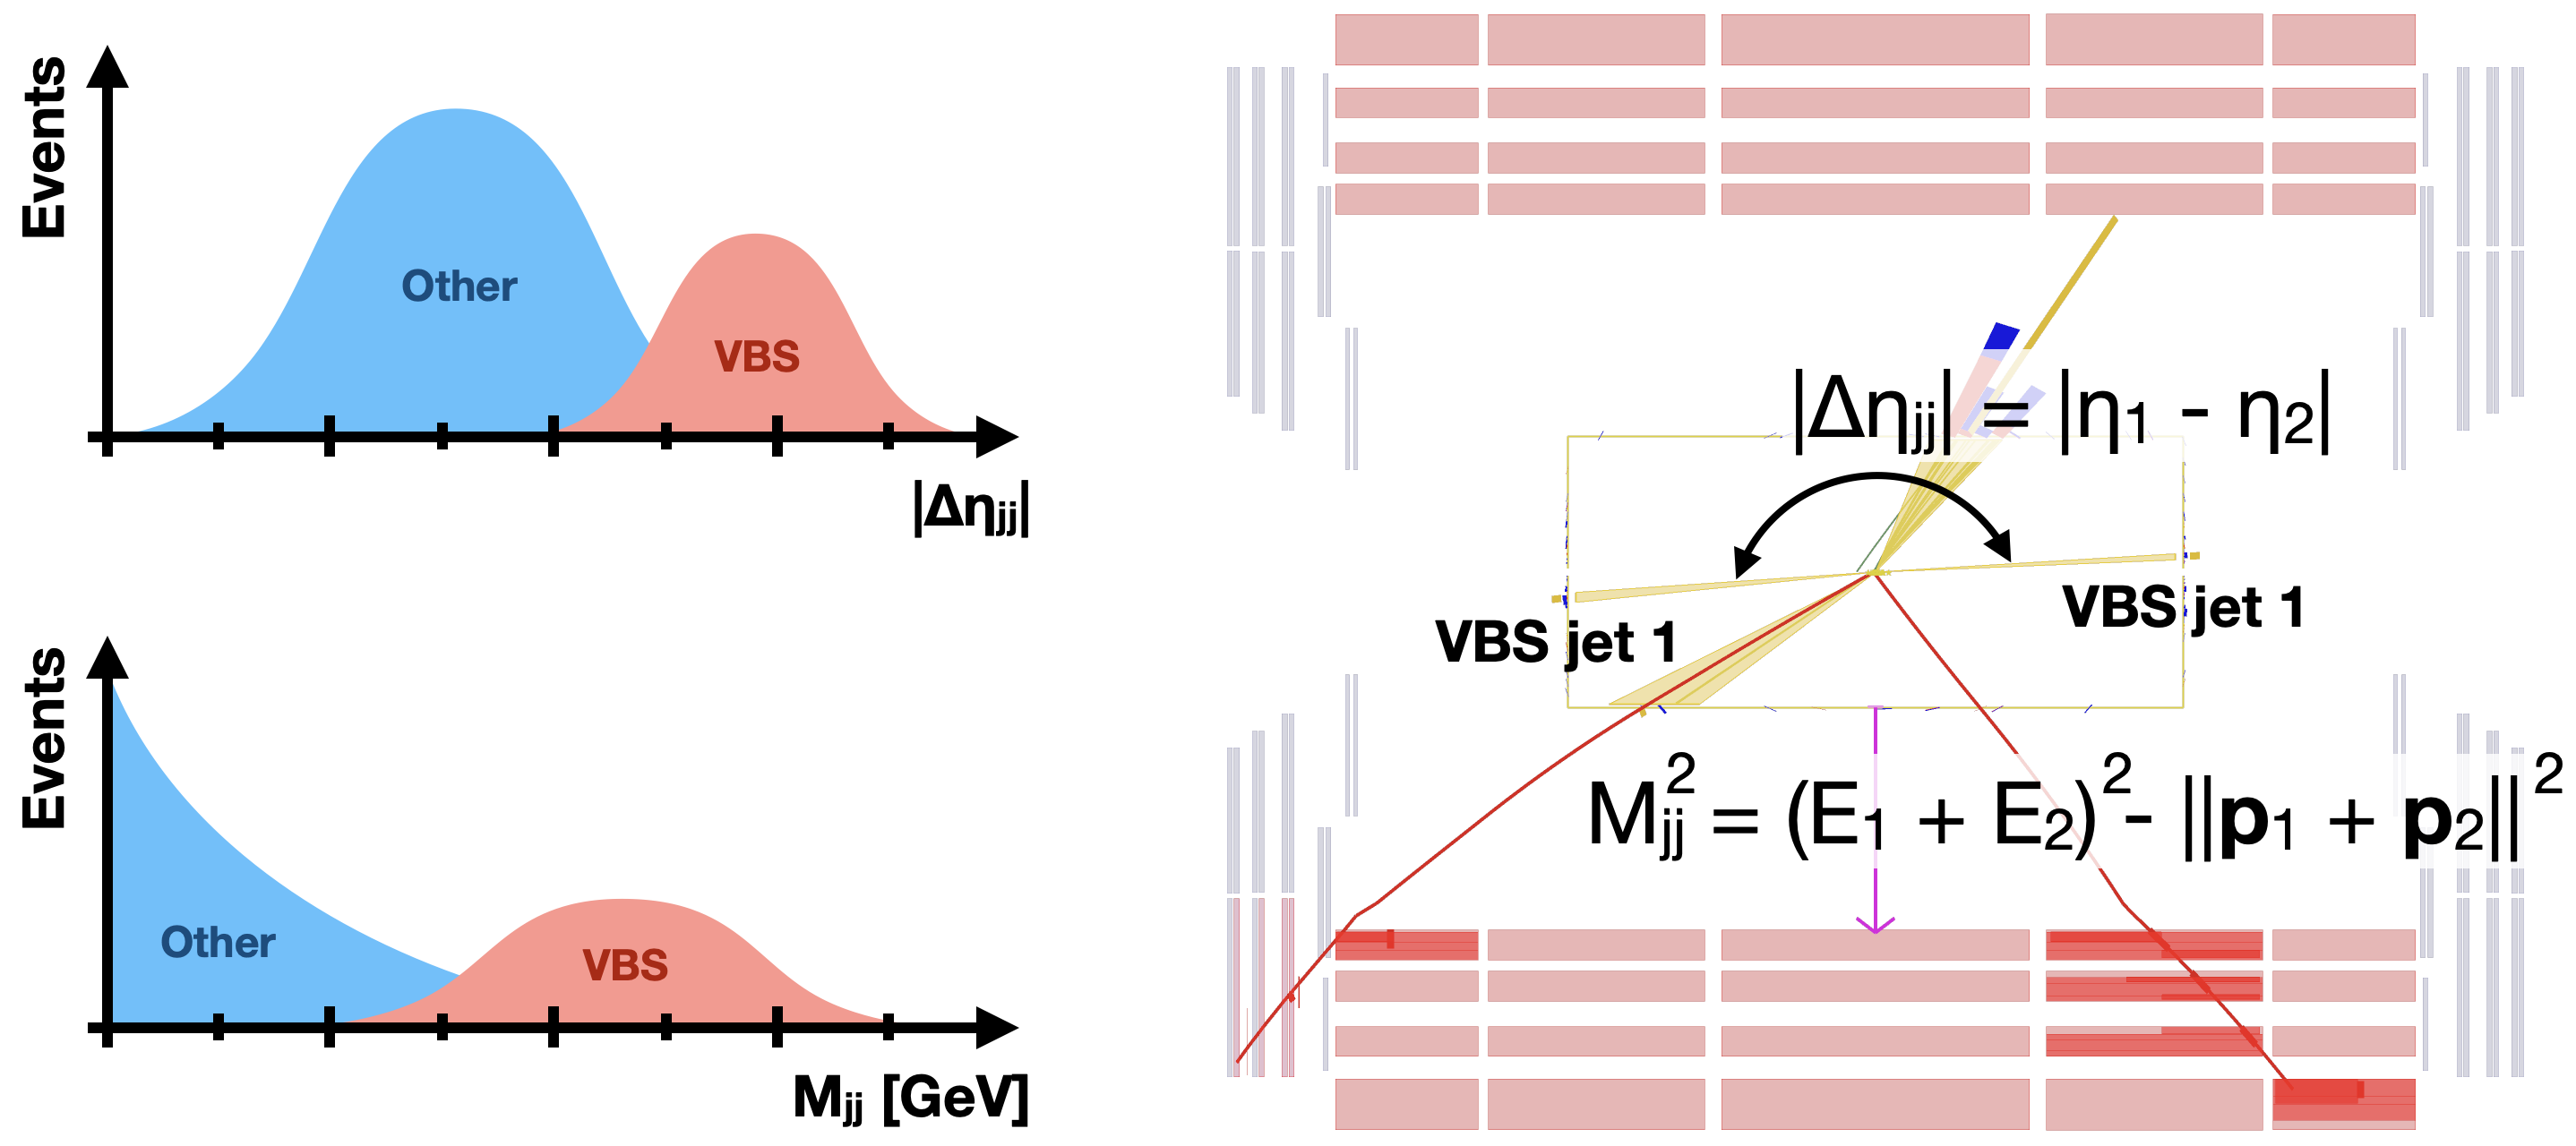
\includegraphics[width=0.9\textwidth]{fig/vbs_signature.png}
    \caption[VBS jets signature]{
        Typical VBS jet \Mjj and $\abs{\detajj}$ distributions (left) next to an event display for a simulated VBS WH signal event in the $r$-$z$ plane, with the VBS jets labeled (right). 
    }
    \label{fig:vbs_fireworks}
\end{figure}

VBS provides a unique way of producing Higgs bosons, with an easily identifiable signature, and there are myriad VBS processes involving a Higgs, each involving different couplings. 
The rarer couplings are of particular interest, including the $\HHVV$ and $\HHH$ couplings (Ch.~\ref{ch:vbsvvh}). 
Also of interest are some of the more obscure properties of the Higgs boson, like the relative sign between the $\HWW$ and $\HZZ$ couplings (Ch.~\ref{ch:vbswh}). 
In all of these measurements, if we confirm SM predictions, we exclude possible BSM directions, and if we find a significant deviation from the SM, we will have opened an entirely new chapter of physics. 

We begin by selecting the Feynman diagrams that involve the couplings of interest---here, we focus on VBS processes. 
We call the selected processes our ``signal.'' 
For example, if we are interested in $\HHVV$, as in Ch.~\ref{ch:vbsvvh}, our signal might be VBS production of a Higgs boson and two vector bosons. 
We must then find our signal, which is often incredibly rare, amongst petabytes of data recorded by CMS. 

\section{Choosing a final state}
The final collection of particles that are actually recorded by CMS are called the ``final state.'' 
As covered in Chapter~\ref{ch:lhc_cms}, Section~\ref{sec:cms}, CMS can record electrons, photons, hadrons, and photons. 
Higgs bosons, vector bosons, gluons, and tau leptons decay to these particles. 
Therefore, when we say we are looking for VBS production of a Higgs boson and two vector bosons, we are really looking for two quarks (VBS) and the decay products of the bosons. 
Some final states are preferable over others, however. 
For convenience, we often prefer to look for \Htobb, since it occurs 58\% of the time---the next-largest ``branching ratio'' is $\PH\to\PWp\PWm$ at 21\%. 
The choice for the decay of the vector bosons is less clear. 
The leptonic decays ($\PW\to\Pell\PGn$ or $\PZ\to\Pellp\Pellm$) are more unique, but are rarer. 
On the other hand, the hadronic decays ($\PV\to\qq$) are more plentiful, but are difficult to distinguish from far more abundant processes. 
The \textit{reconstruction} of the final state of each proton-proton collision, based on the electronic readout of CMS, is thus crucial for the entire physics operation at CMS---and any other experiment at the LHC. 
Importantly, many SM particles decay to neutrinos, which pass through CMS completely undetected, and it is possible that BSM particles are similarly missed, but the presence of these particles can be inferred if the reconstruction is performed with high precision. 

\section{Reconstruction}
The subdetectors that comprise CMS produce a set of electric signals digitized into data that can be used as measurements of physical quantities. 
Moreover, when associated to one another, these measurements can also be used to ascertain the identity of detectable throughgoing particles (Fig.~\ref{fig:cms_particle_id}). 
This is done via a global ``particle-flow'' (PF) algorithm~\cite{CMS:2017yfk}, which combines the information from each of the CMS subdetectors to reconstruct all individual particles in an event. 
Particles reconstructed by the PF algorithm are called PF ``candidates'' and are used to build jets, which originate from hadrons, \PGt leptons, and in the computation of the missing transverse momentum (\ptmiss). 

\begin{figure}[htb]
    \centering
    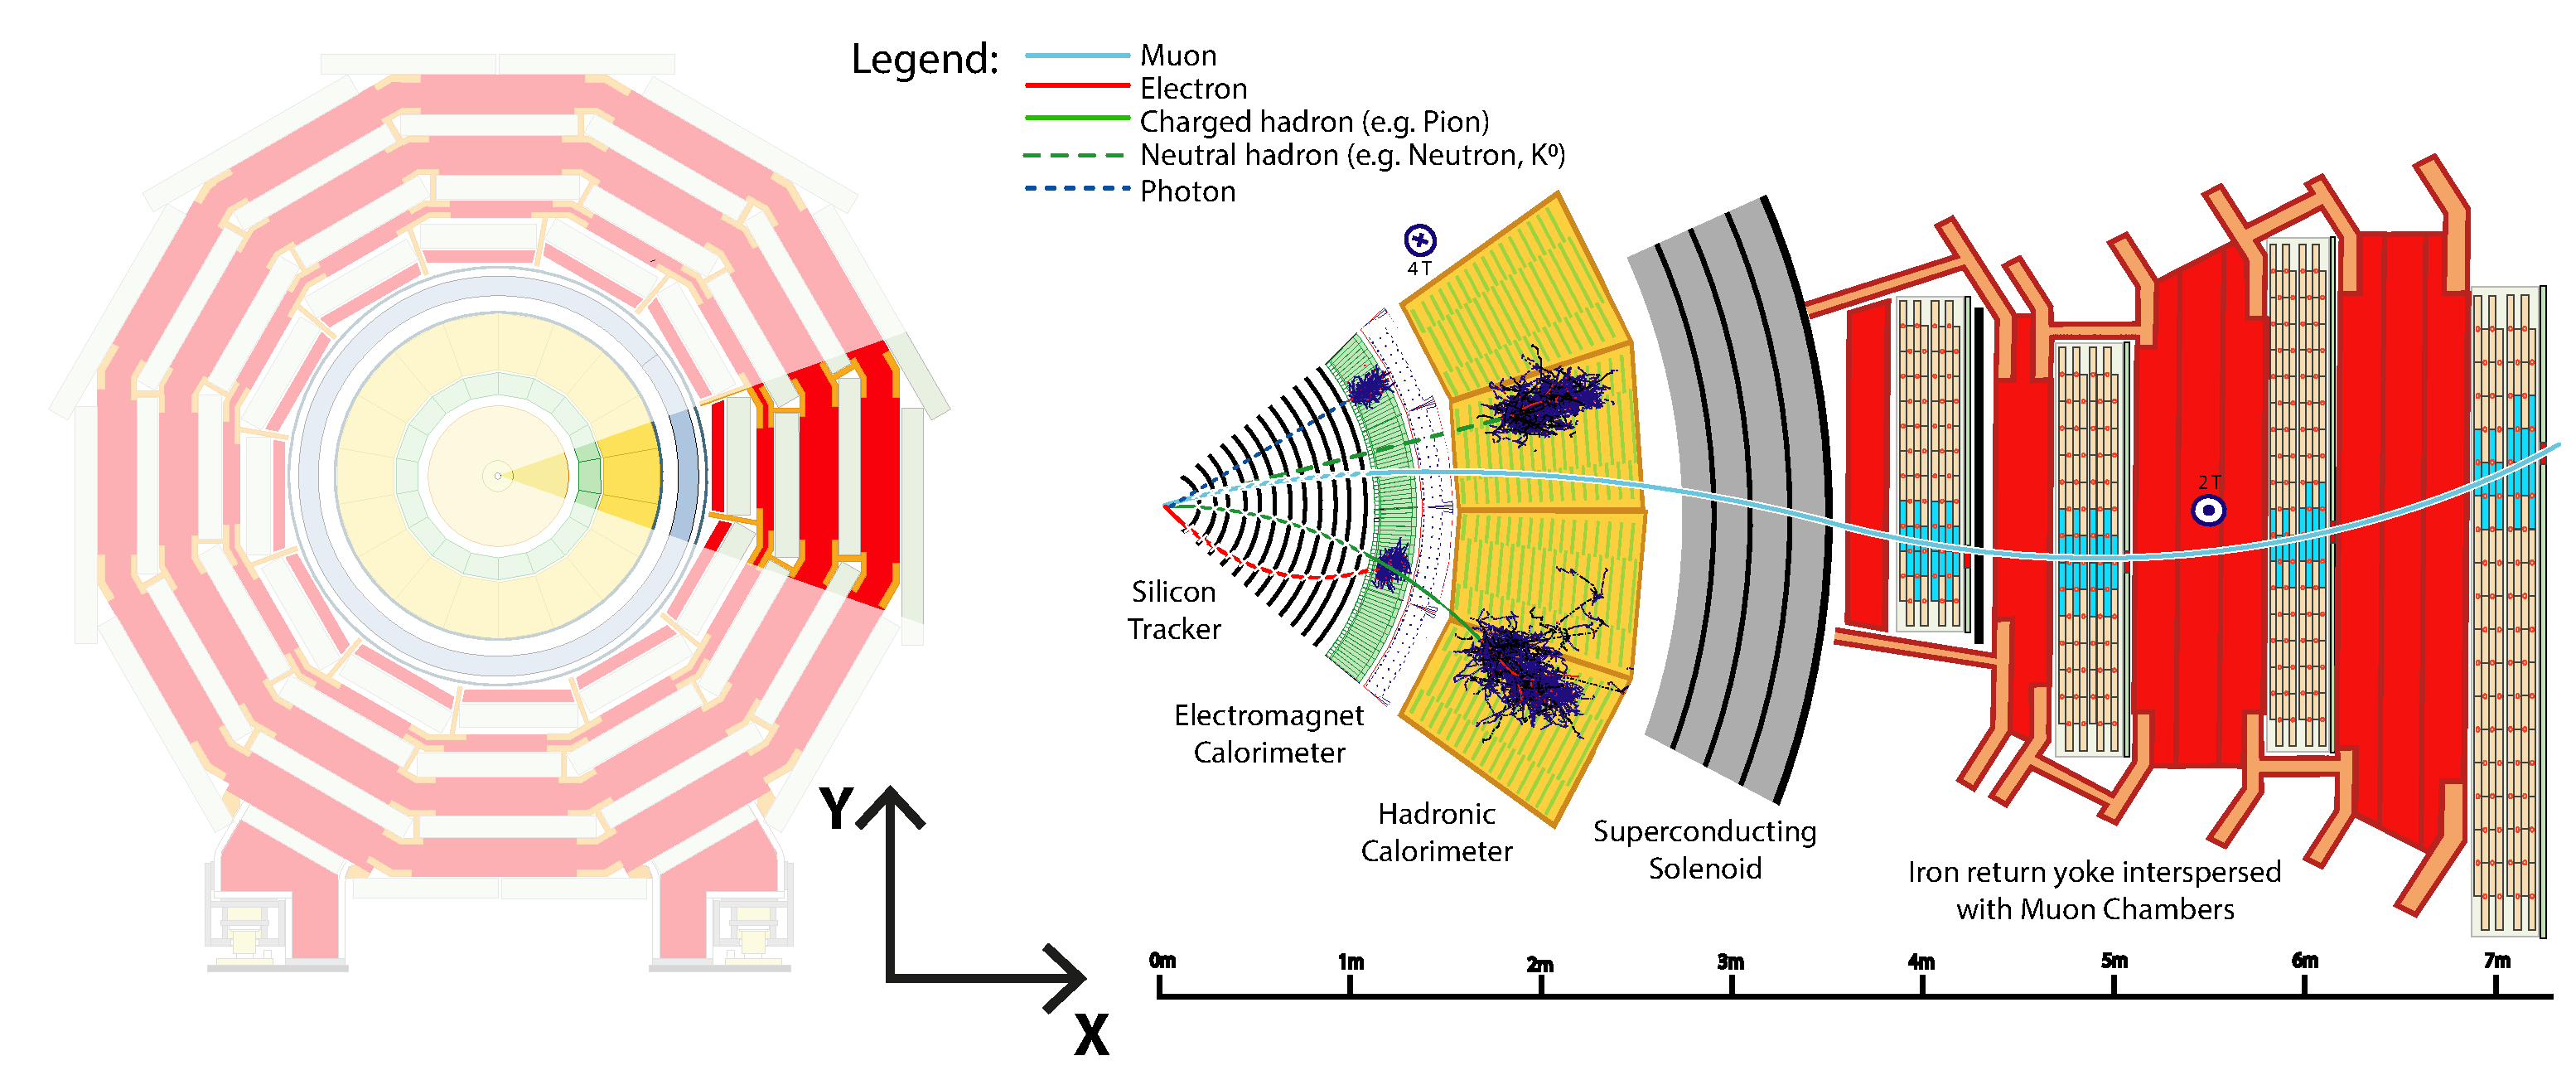
\includegraphics[width=0.95\textwidth]{fig/cms/particle_id_slice.pdf}
    \caption{
        Transverse slice of CMS, from Ref.~\cite{Davis:2205172}, showing the signals left by different kinds of particles in each subdetector.
    }
    \label{fig:cms_particle_id}
\end{figure}

\subsection{Jets}
All hadrons leave a hit in the HCAL, while charged hadrons also have a track that can be associated to it, but these hits do not correspond to individual quarks---like the VBS quarks, for example. 
Due to quark ``confinement,'' quarks hadronize into ``jets'' of hadrons. 
This happens in a cascade, where quarks beget quarks that beget more quarks and so on, until the jet impinges on the calorimeters. 
Fortunately, jets tend to be concentrated in relatively narrow cones, meaning individual jets---and thus, individual quarks---can usually be distinguished from one another. 
Jets are constructed using the anti-\kt algorithm~\cite{Cacciari:2008gp, Cacciari:2011ma}, which clusters PF candidates according to a configurable ``distance parameter,'' which determines the size of the jet cone. 
For AK4 jets, the distance parameter is set to 0.4, corresponding to $\DeltaR = 0.4$, where
\begin{equation}
    \DeltaR = \sqrt{\Delta\phi^2 + \Delta\eta^2}
\end{equation}
There is also a collection of AK8 jets, which have the distance parameter set to 0.8, which captures merged jets.

\subsubsection{Jets originating from \Pb quarks}
While the presence of quarks can be inferred from the presence of jets, the identity (flavor) of each quark is less obvious. 
However, when \Pb quarks hadronize, they produce a B meson (Fig.~\ref{fig:btagging_step1}). 
The B meson lifetime is sufficiently long such that it passes the first few layers of the tracker before decaying---only picoseconds after it was produced. 
When it decays, it produces several quarks and, potentially, a lepton. 
This results in ``displaced'' tracks in the tracker that point to a ``secondary vertex'' (Fig.~\ref{fig:btagging_step2}) as opposed to the ``primary vertex,'' or the original pp collision. 
The presence of a secondary vertex within a jet therefore gives a unique indication that it originated from a \Pb quark (Fig.~\ref{fig:btagging_step3}). 
Particle tracks are therefore vital for \Pb-tagging, so \Pb-tagged jets must be within the tracker acceptance region ($\abs{\eta} < 2.5$). 
For CMS analysis, a deep neural network called \DeepJet was trained to use the presence of a secondary vertex, along with additional kinematic information about the jet and its constituents, to ``tag'' jets as originating from a \Pb quark~\cite{Bols:2020bkb}. 

\begin{figure}[htb]
    \centering
    \subfloat[]{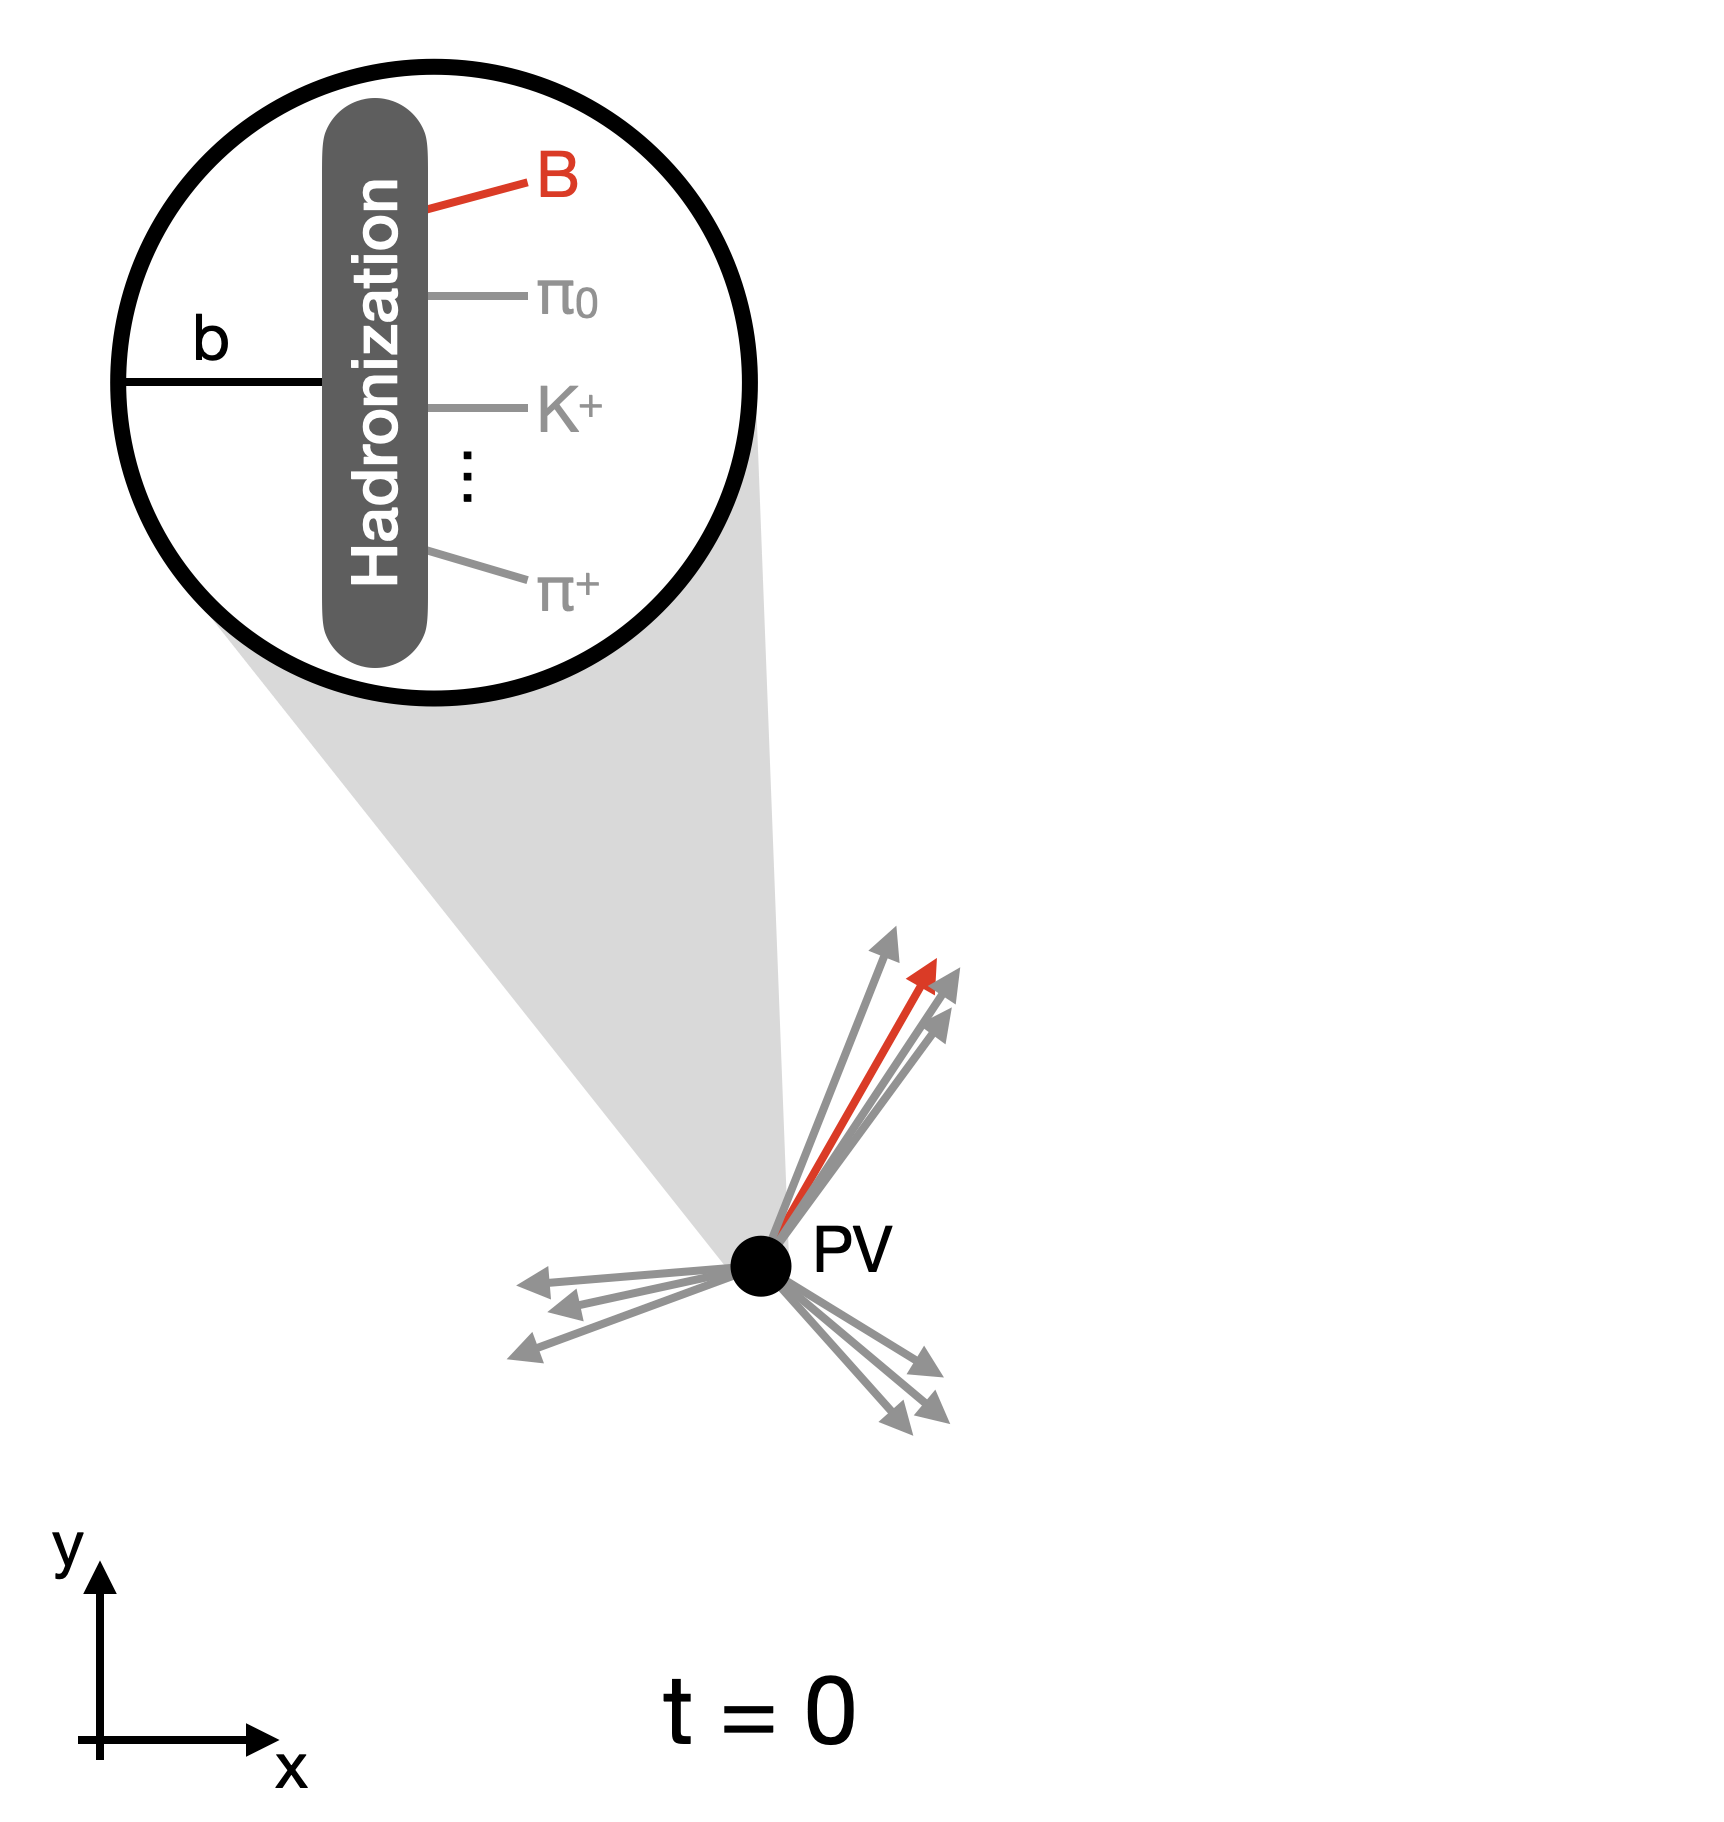
\includegraphics[width=0.33\textwidth]{fig/cms/btagging_step1.png}\label{fig:btagging_step1}}
    \subfloat[]{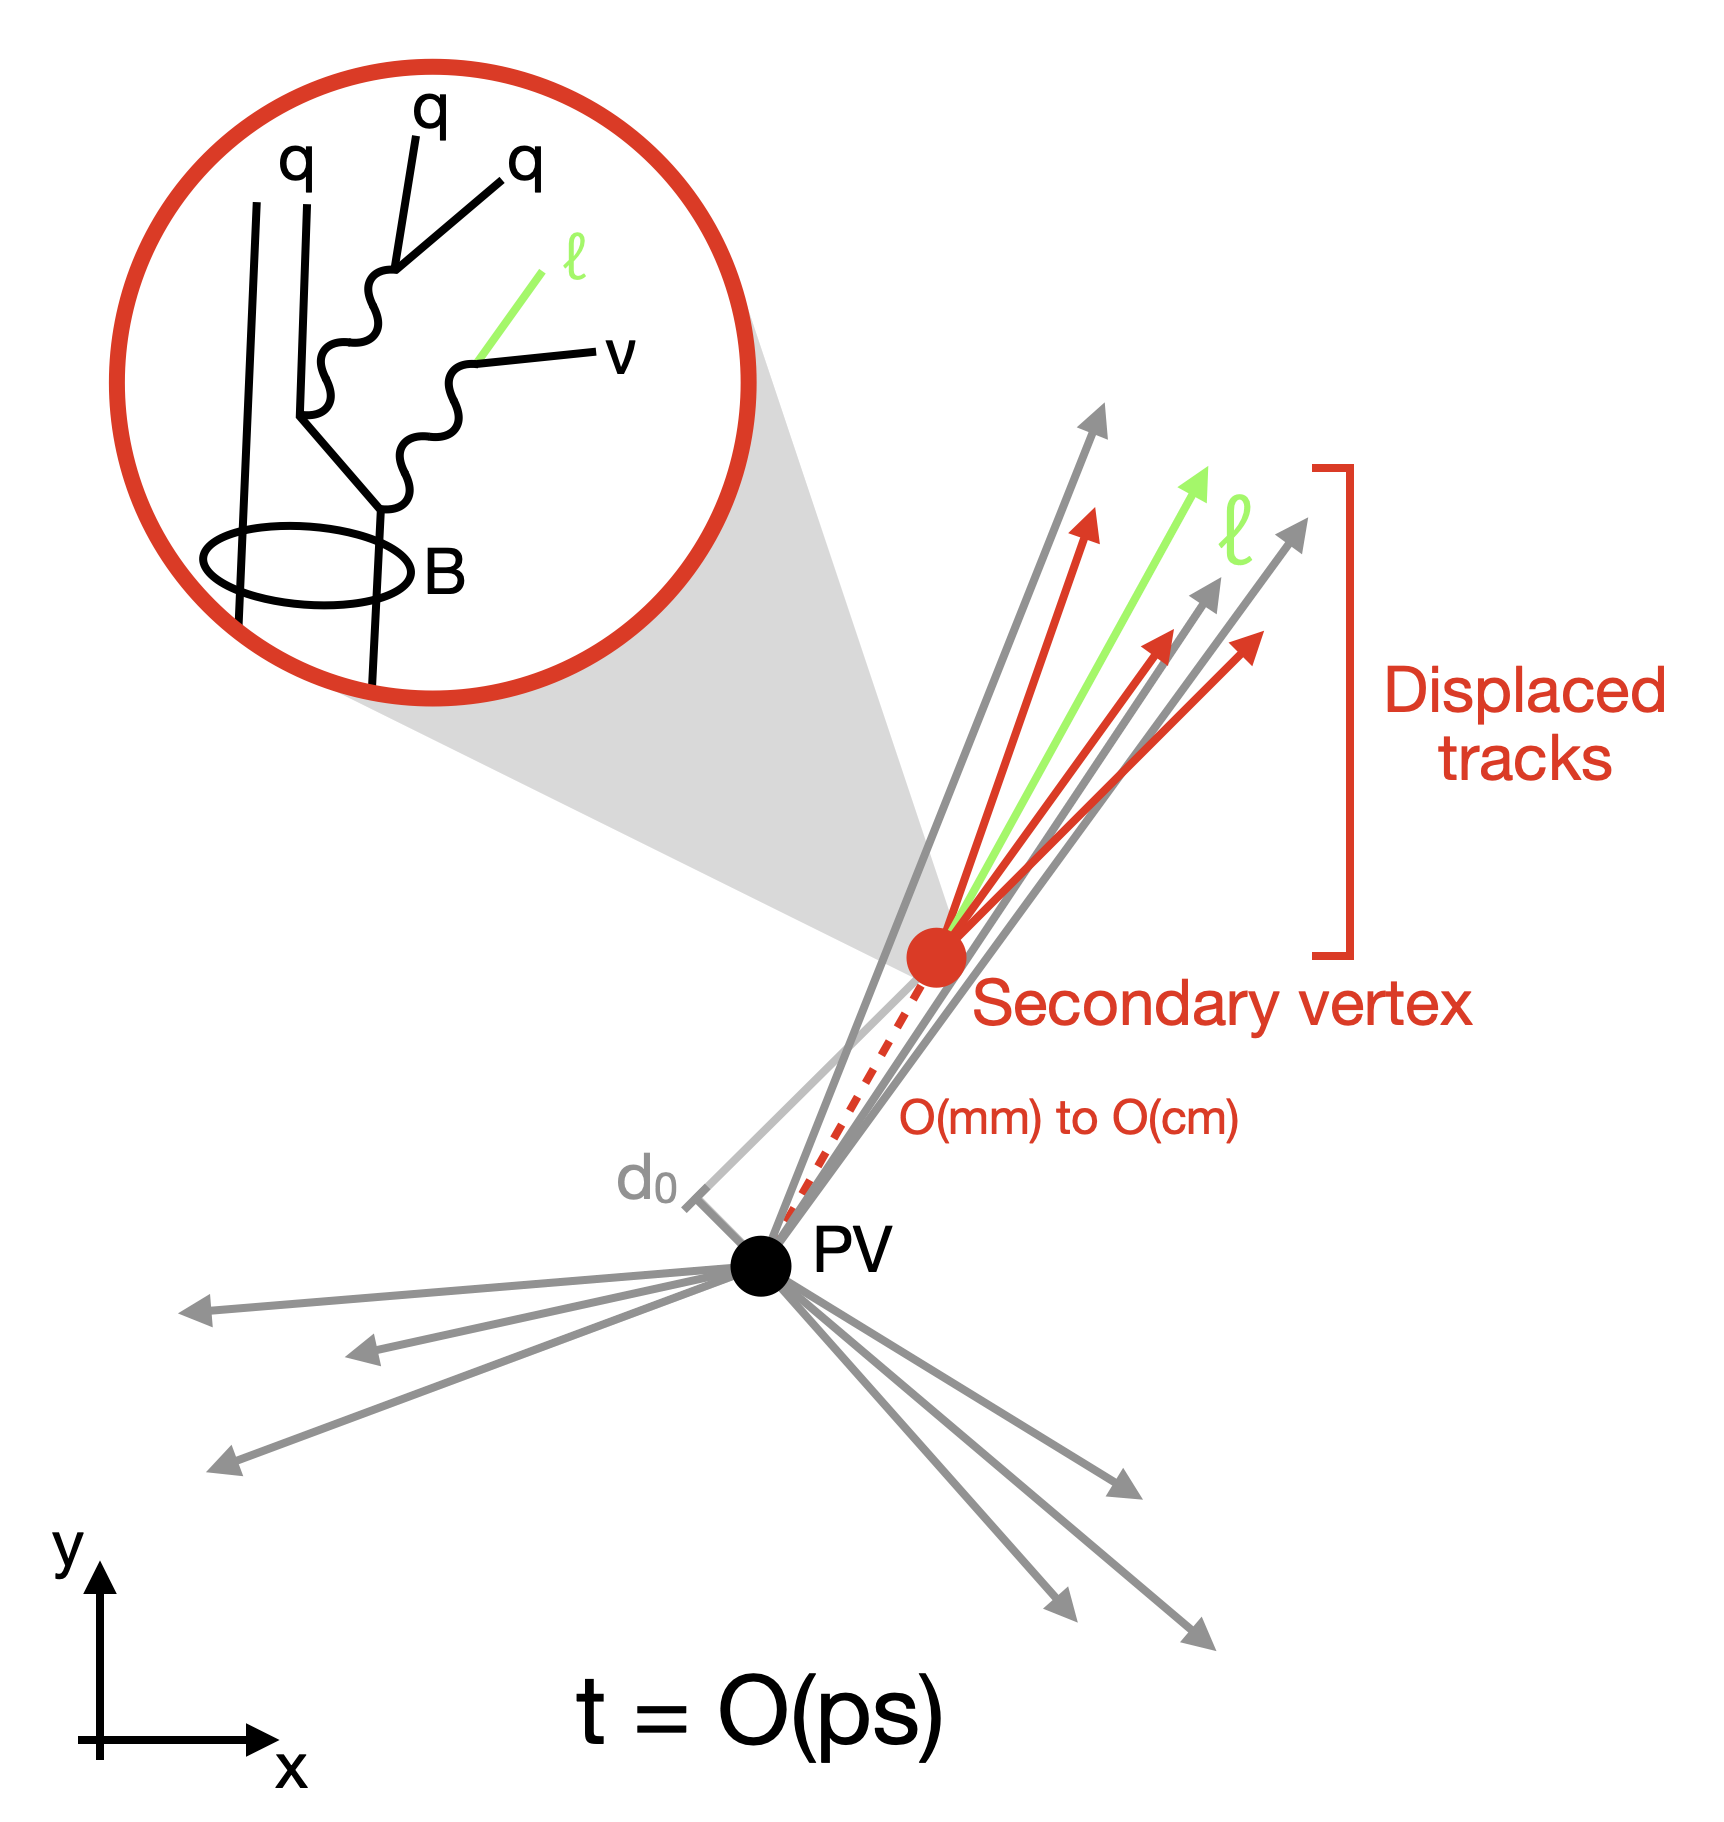
\includegraphics[width=0.33\textwidth]{fig/cms/btagging_step2.png}\label{fig:btagging_step2}}
    \subfloat[]{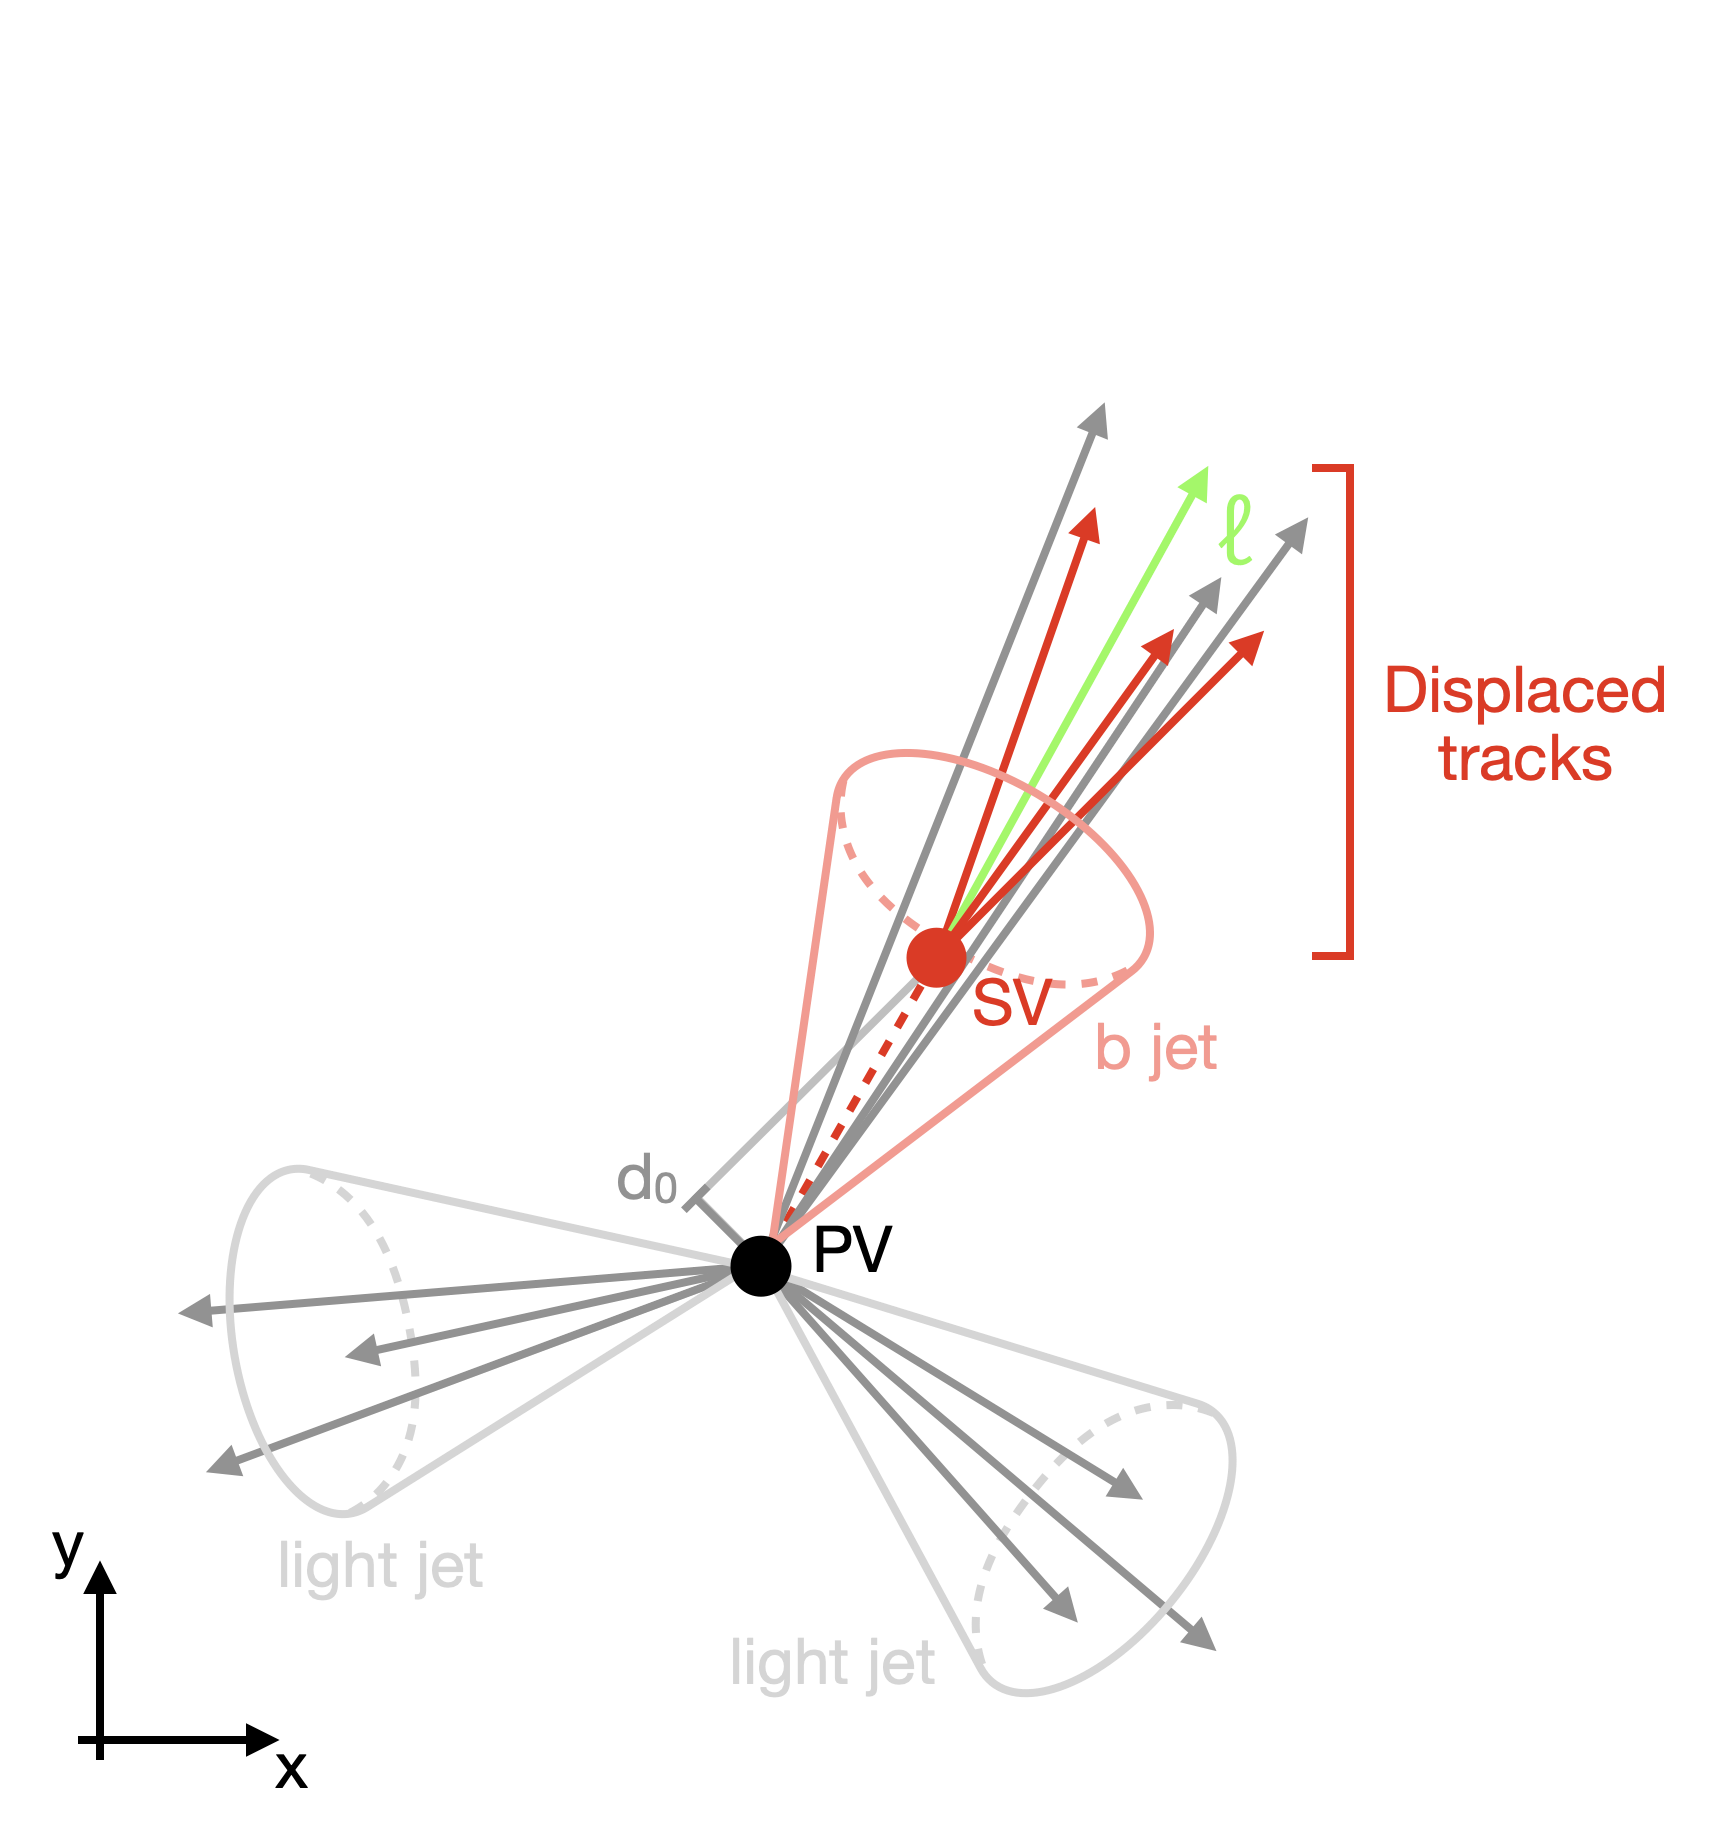
\includegraphics[width=0.33\textwidth]{fig/cms/btagging_step3.png}\label{fig:btagging_step3}}
    \caption[A sketch of the hadronization and identification of a \Pb quark]{
        A sketch of the hadronization of a \Pb quark (left), the subsequent hadronization of the produced B meson (center), and the identification of each jet (right). 
        Based on Ref.~\cite{BTaggingDiagramOrig}.
    }
    \label{fig:btagging}
\end{figure}

\subsubsection{Merged jets originating from \Htobb}
In cases where a highly energetic particle decays to a pair of quarks, the resulting jets overlap or are near enough to each other to be difficult to separate. 
This presents a unique signal: the two nearby jets can instead be found as a single, large-cone jet. 
That is, these merged jets will appear in the AK8 jet collection. 
In the work presented in this dissertation, we search for Higgs bosons decaying to \bbbar at high energies, tagged as a single merged jet. 
This is made possible by a graph neural network, called \ParticleNet, trained for CMS analysis to identify the origins of merged jets based on the properties of its constituents, arranged in a graph-like data structure according to their proximity to one another~\cite{Qu:2019gqs}. 
Similar to \Pb-tagging, merged jets considered for \Xtobb tagging, for instance, must be within the tracker acceptance region. 
The merged jet with a mass similar to the Higgs boson, and the highest \ParticleNet \Xtobb score is considered as the best Higgs boson candidate.

\subsubsection{Jets originating from VBS quarks}\label{sec:vbsjets}
The presence of VBS quarks is inferred from the presence of two jets that are back-to-back (large $\abs{\detajj}$) and have a large combined invariant mass (\Mjj). 
In events where there are more than two additional jets that do not overlap with the Higgs boson candidate jet, the two best VBS jet candidates must be selected. 
A unique VBS selection technique was derived for the work presented in this dissertation: 
if all of the jets are in one hemisphere of $\eta$, then the two jets with the largest momenta are selected; 
otherwise, the jet with the largest momentum in each $\eta$ hemisphere are selected. 

\subsection{Leptons}
For simplicity, when we consider ``leptons,'' we will exclusively mean those leptons that are directly detected by CMS, namely electrons and muons. 
Electrons have a track in the silicon tracker and leave a deposit in the ECAL. 
The tracks and ECAL deposit can be associated to one another, distinguishing electrons from photons, which only leave a deposit in the ECAL. 
Muons also have a track, but they fly past both calorimeters undetected and leave hits behind in the muon chambers. 

In the SM, the lepton family also includes tau leptons and neutrinos. 
Tau leptons decay almost immediately to hadrons or to a tau neutrino and \PW boson. 
The latter decay is difficult to reconstruct, because it is easily confused with a lone \PW boson. 
The hadronic decay, however, has a unique ``multi-prong'' structure, allowing it to be distinguished from other jets. 
Neutrinos, meanwhile, pass through the entire detector, so their presence can only be inferred by first accounting for everything else, then asking for what is missing. 

\subsection{Missing energy}\label{sec:met}
Protons collide along the beamline with equal but opposite momenta, so the system has a total momentum of zero. 
Because of the conservation of momentum, the sum of the momenta of all produced particles must still be zero. 
This is as true in the classical world as the quantum world. 
The shrapnel from two colliding bullets, for instance, is thrown from the collision in a disk, so the total momentum is conserved~\cite{SmarterEveryDayBullets}. 
Therefore, if an invisible particle (a neutrino or possibly something new) is produced, its momentum will not be recorded, and the sum of momenta will be non-zero. 
Since the missing momentum will be entirely in the transverse plane, the plane perpendicular to the beamline, it is referred to as \ptmiss, or missing transverse momentum. 

\section{Identifying backgrounds}
Of course, final states are not unique. 
For example, if we were searching for $\PZ\to\Pellp\Pellm$, and thus asked for collision events with two leptons with opposite charge, we would also get events where a \PWp and \PWm were produced and both decayed leptonically. 
We could also pick up events where \PW and \PZ boson were produced, and both decayed leptonically, but the lepton from the \PW was not recorded by CMS. 
These processes that produce the same final state, but are not the signal, are referred to as ``backgrounds.'' 

One common background for VBS Higgs boson analyses is \ttbar production. 
Both top quarks decay to a \PW boson and \PQb quark. 
With either the hadronic or leptonic decay of the \PW bosons, and the two genuine \PQb jets, there is a large potential for trickery. 
For example, the \PW boson could decay to two quarks that overlap with each other and one of the \PQb jets, resulting in a jet with a large invariant mass and displaced tracks that could be mistaken for a \Htobb jet (e.g. Fig.~\ref{fig:vbs_vs_ttbar}). 
Backgrounds including genuine VBS jets or a genuine Higgs boson are typically much rarer than a more populous background like \ttbar generating a fake signature. 

\begin{figure}[htb]
    \centering
    \subfloat{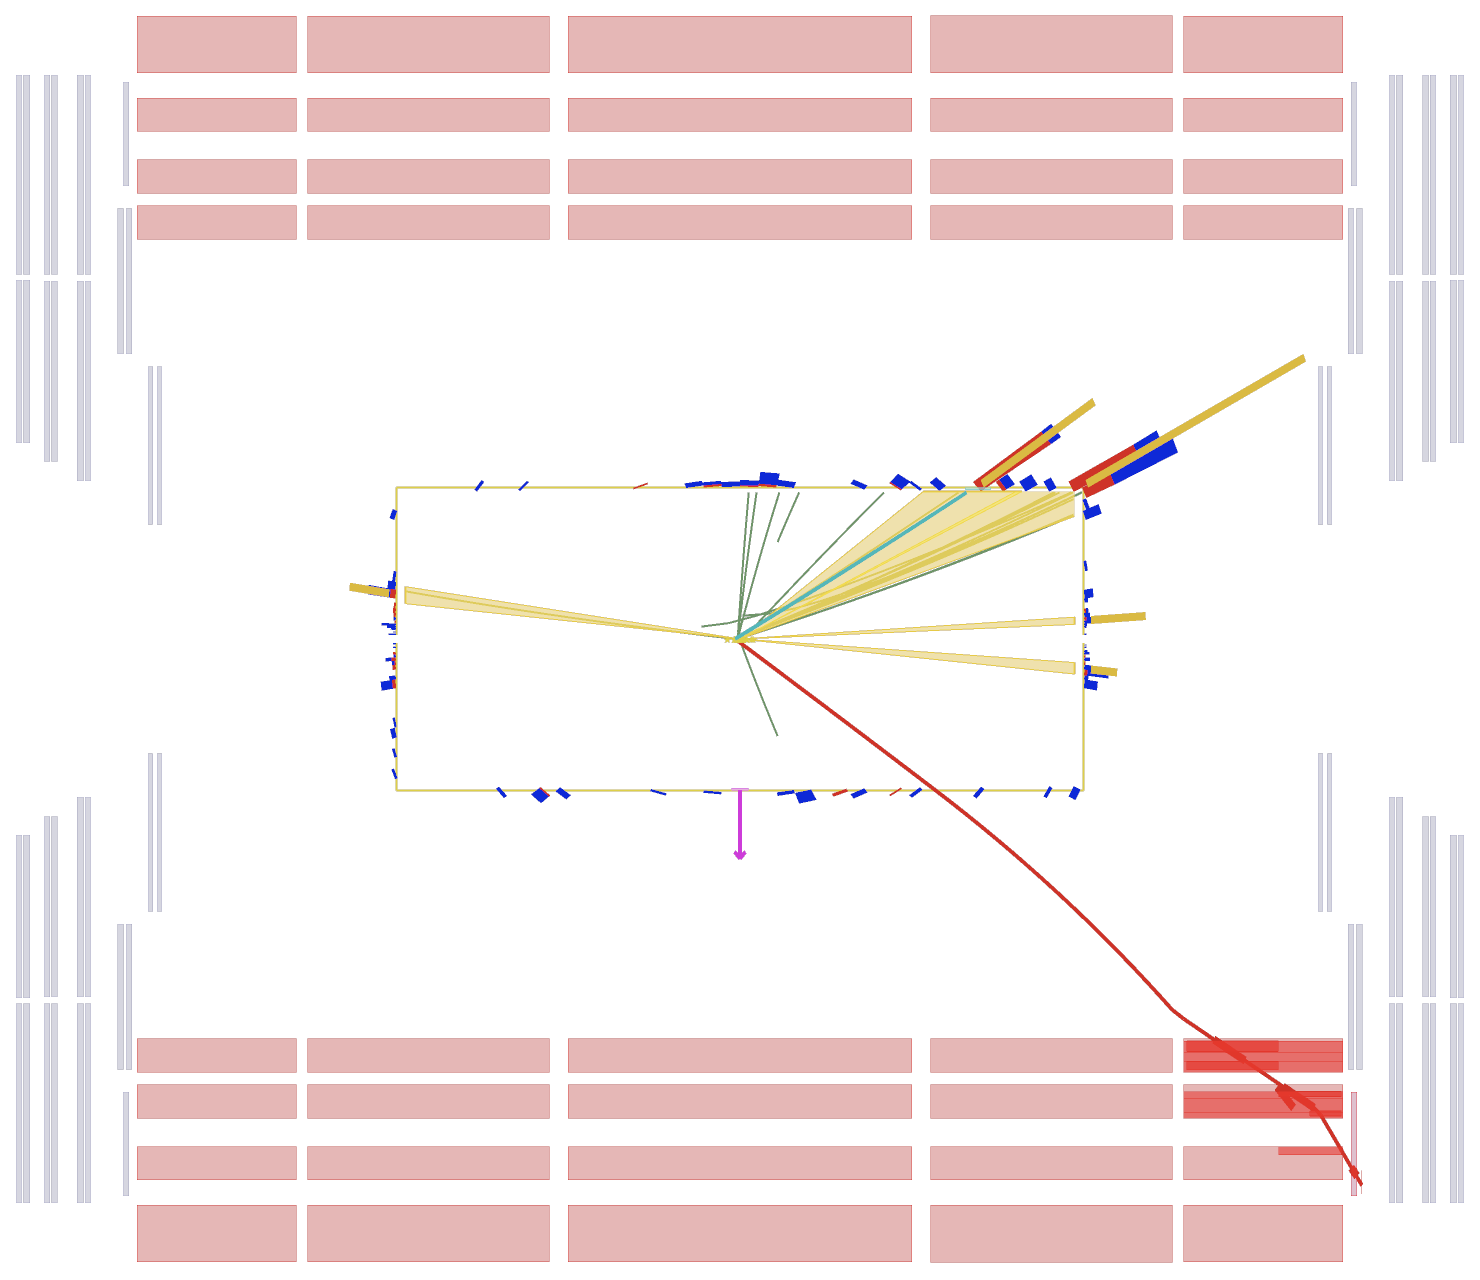
\includegraphics[width=0.45\textwidth]{fig/vbswh/fireworks/signal/vbswh_evt131107_rz.png}}
    \qquad
    \subfloat{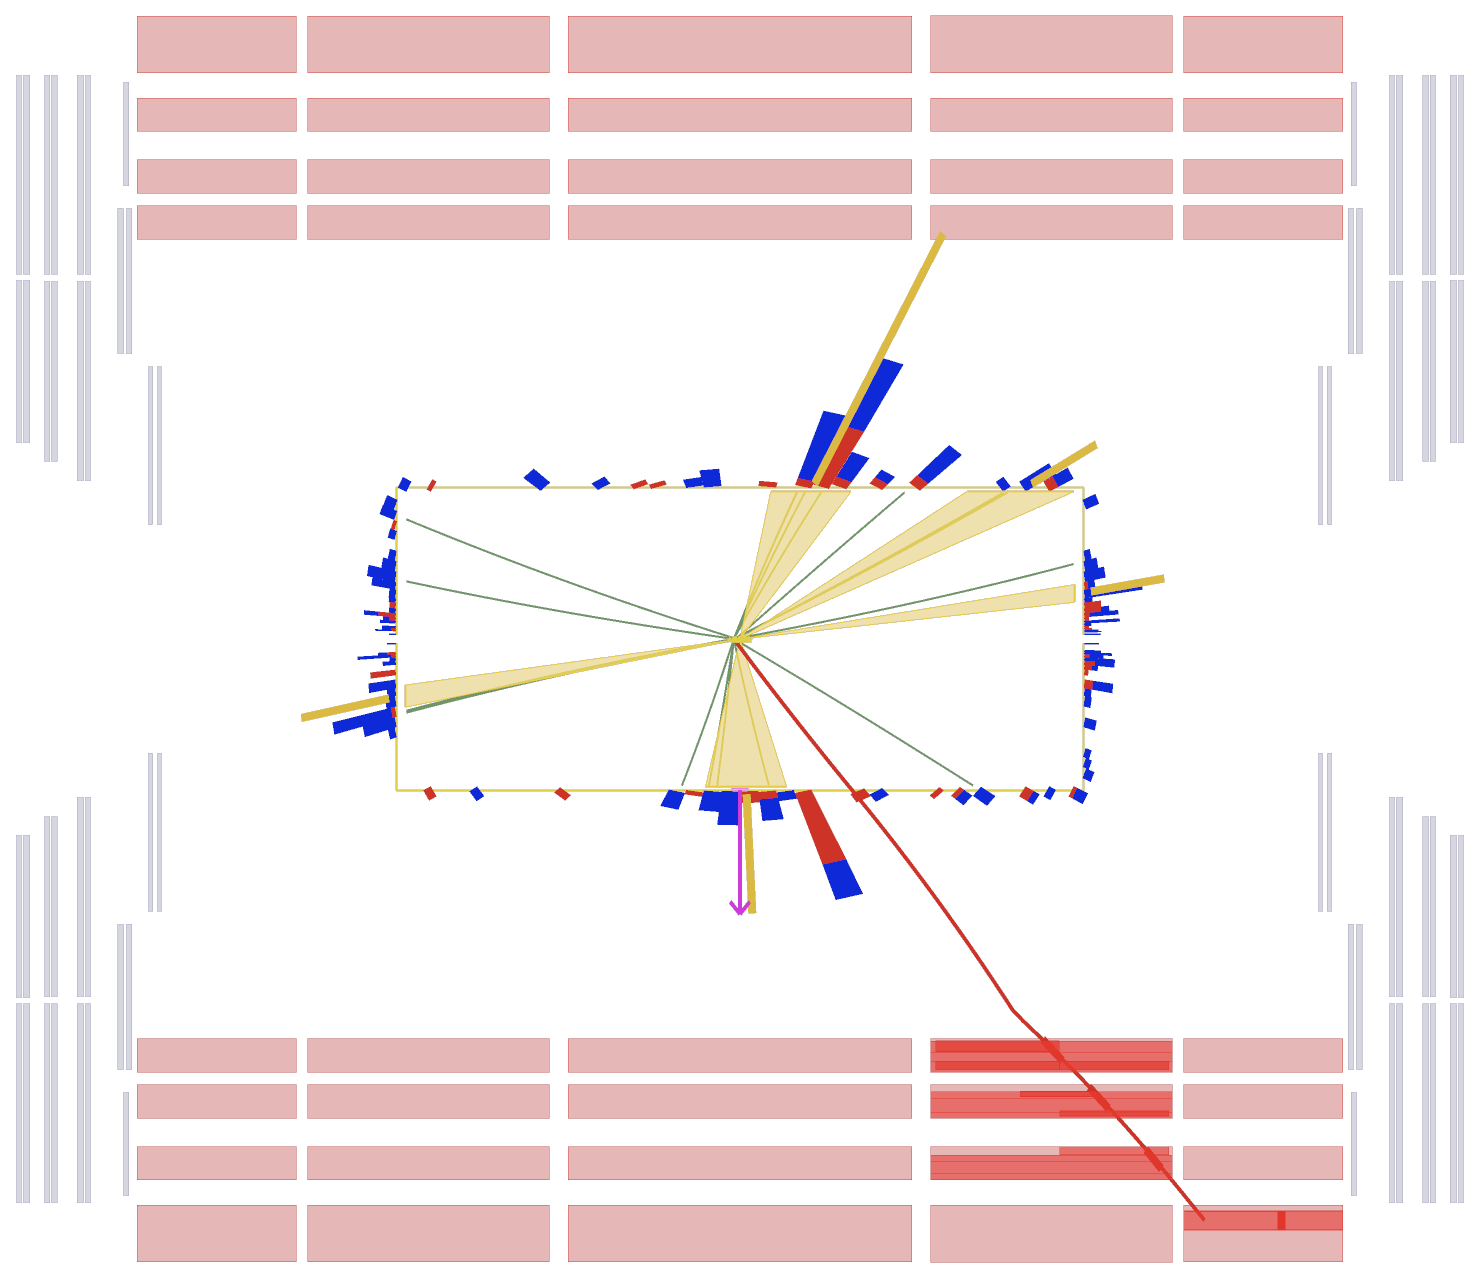
\includegraphics[width=0.45\textwidth]{fig/vbswh/fireworks/bkg/ttbar_rz.png}}
    \caption[Event display for a simulated VBS \WH signal and \ttbar event]{
        Event display for a simulated VBS \WH signal event (left) and \ttbar event (right). 
        Both events contain two forward jets, a single muon, and two \PQb jets. 
    }
    \label{fig:vbs_vs_ttbar}
\end{figure}

\section{Simulation}
Some experiments can control when interesting data is being recorded, so background noise can be directly measured by simply turning the source of interesting data off, but leaving the experiment on. 
The CMS Experiment does not have this luxury: interesting collision events are buried amidst billions of uninteresting ones---the L1 trigger and HLT only make very general selections. 
Moreover, as covered in the previous section, the signal final state is not unique, so although the PF algorithm is capable of reconstructing each particle produced in a proton-proton collision, we must carefully examine those produced by signal versus background such that we may separate them in our analysis. 
This cannot be done easily using only data, since we do not know a priori what really happened---we can only know what was produced. 
Instead, we use Monte Carlo (MC) simulation software that ``generates'' proton-proton collisions, where we can specify exactly what physics processes occur~\cite{Buckley:2011ms}. 

\begin{figure}[htb]
    \centering
    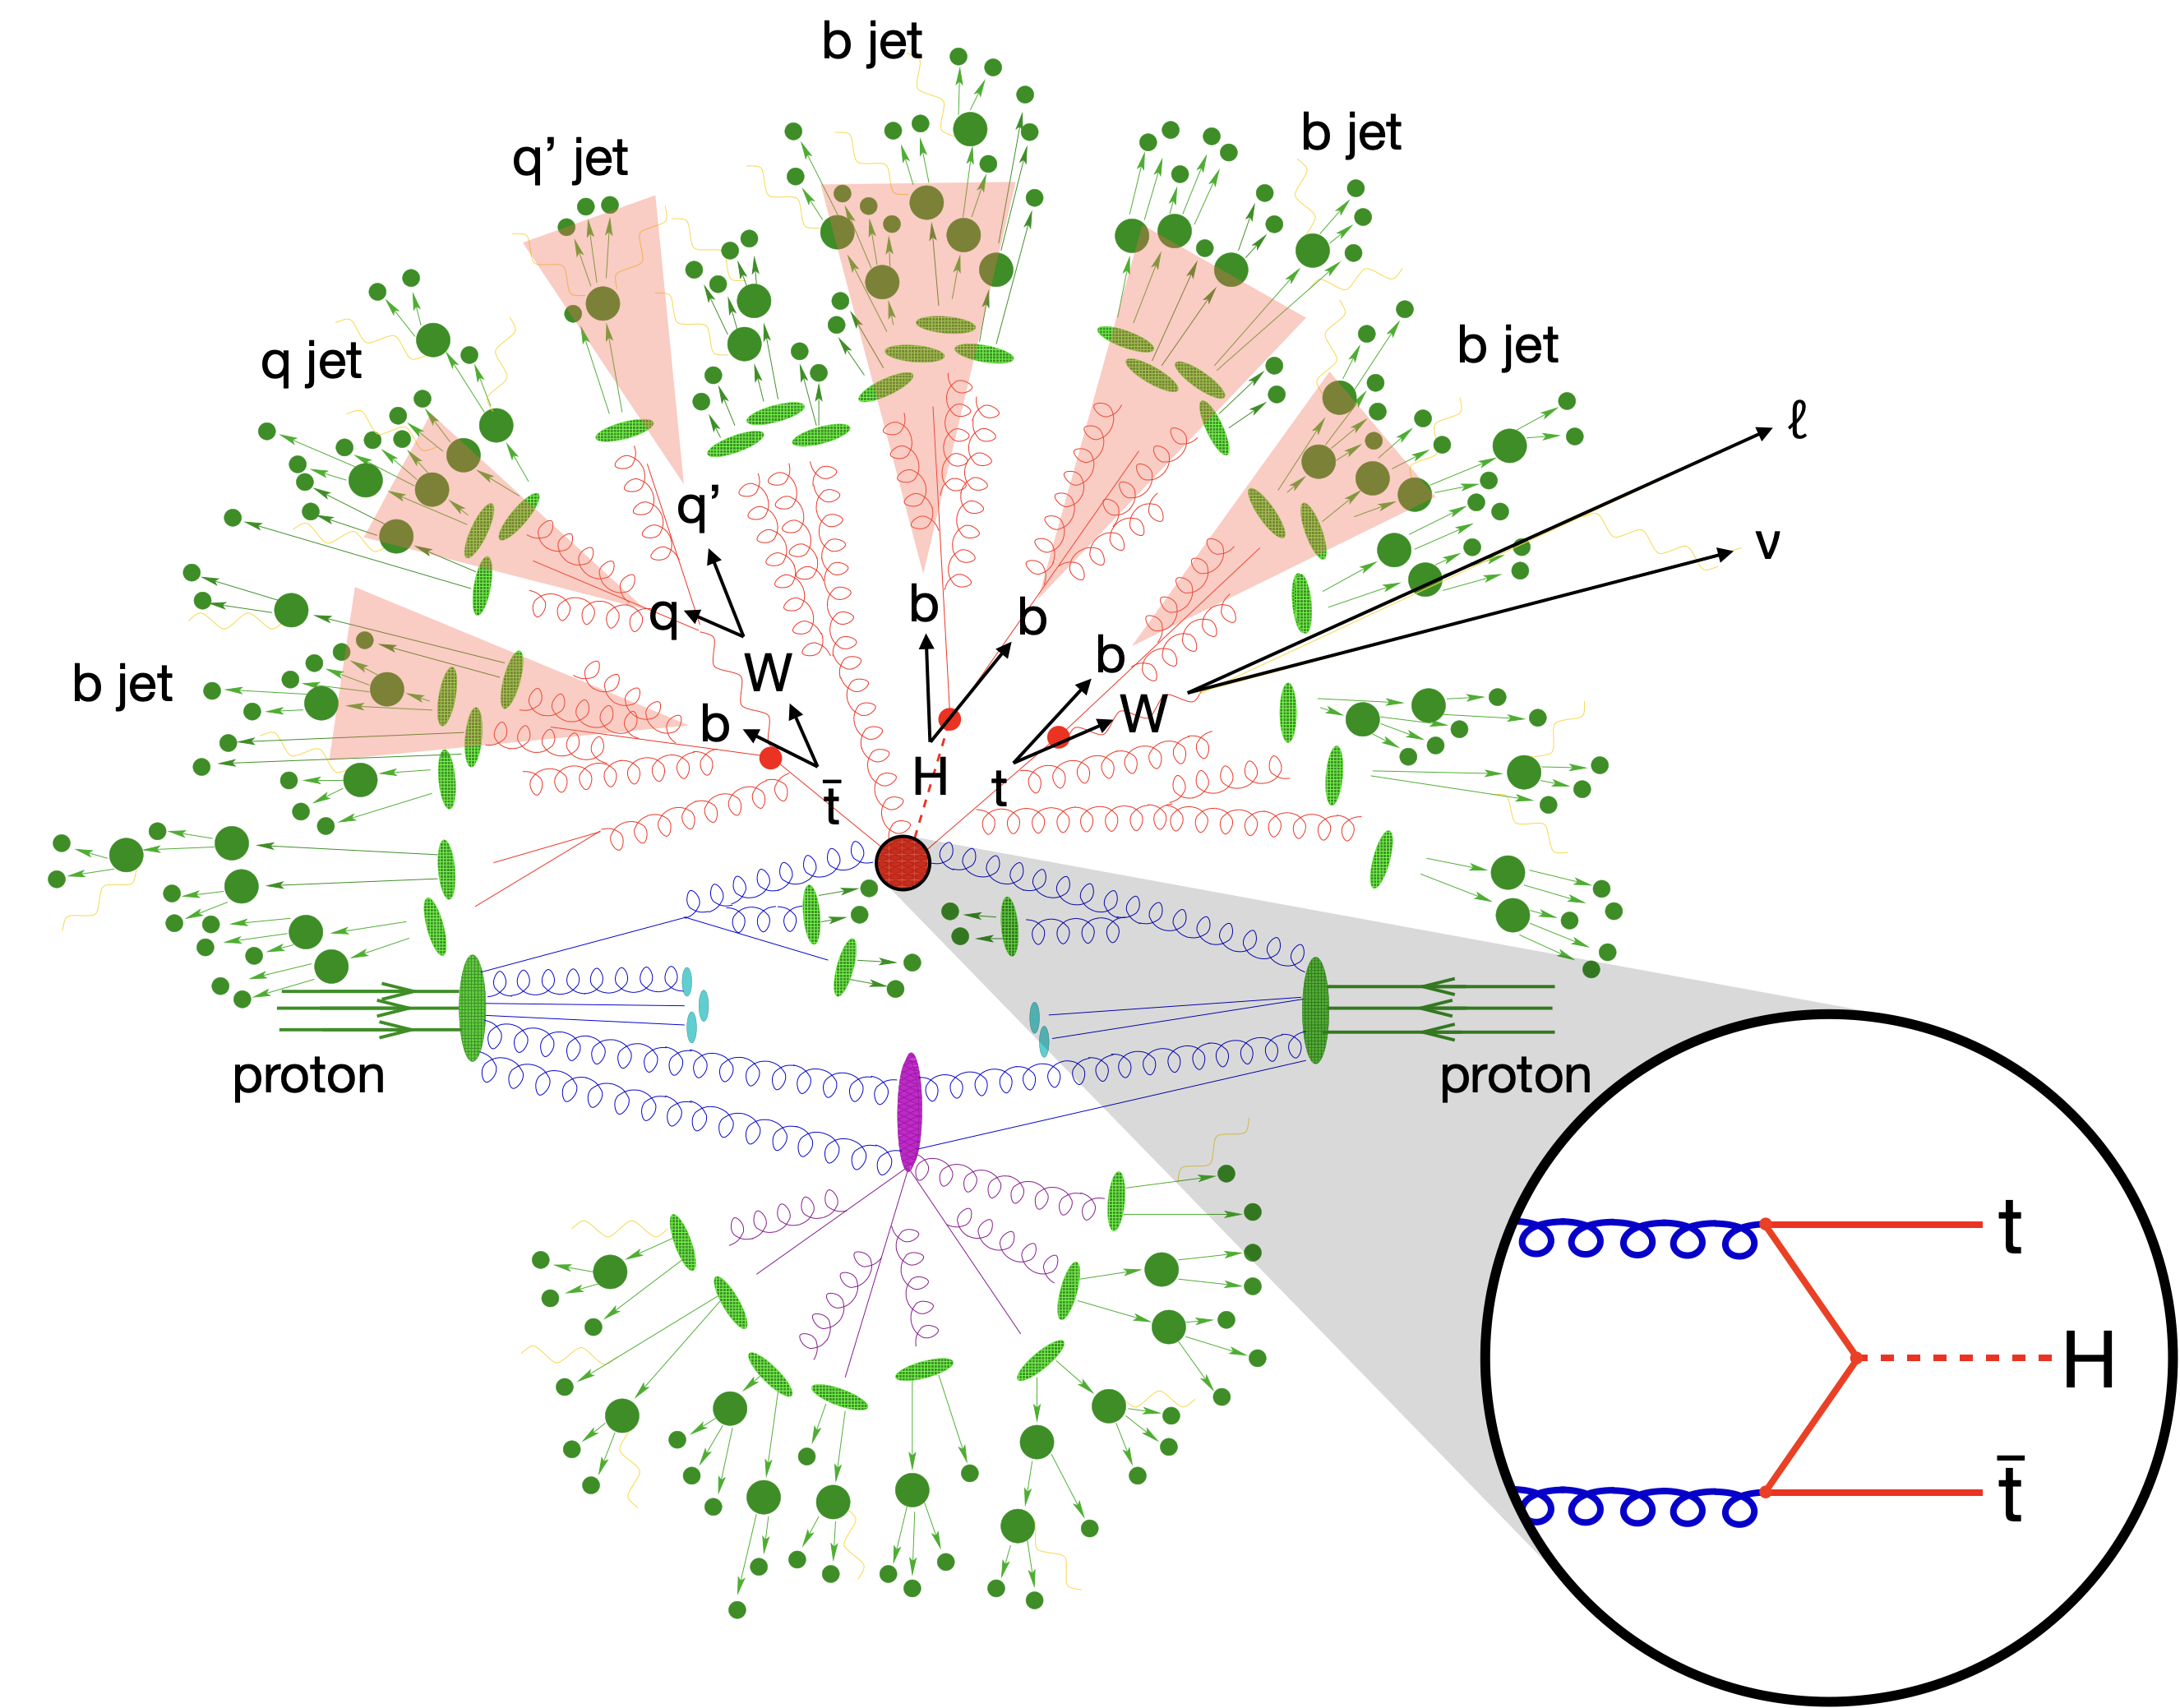
\includegraphics[width=0.85\textwidth]{fig/mc_diagram_labeled.png}
    \caption[Detailed diagram of the generation of a single $\Pp\Pp\to\ttbar+\PH$ event]{
        Detailed diagram of the generation of a single $\Pp\Pp\to\ttbar+\PH$ event, based on Ref.~\cite{Gleisberg:2008ta}, starting from hard scattering (circled), to the decay of the top quark, anti-top quark, and Higgs boson (black arrows and text), to the hadronization of the final state into jets (red triangles). 
        Also included are jets from final-state radiation, i.e. gluons radiated from the final state quarks, and initial-state radiation, i.e. jets from the other constituents of the colliding protons. 
    }
    \label{fig:ttbarH_mc}
\end{figure}

Taking $\Pp\Pp\to\ttbar+\PH$ as an example (Fig.~\ref{fig:ttbarH_mc}), the first step of generating a MC simulation is to calculate the kinematics (the energy and the momentum vector) for the top quark, anti-top quark, and Higgs boson. 
This is often done with the \MGvATNLO ``matrix-element'' generator, which finds the relevant Feynman diagrams, including very rare ones, and randomly generates different realizations of the final state based on an approximation of the underlying theory. % TODO: cite MadGraph AMC@NLO paper
Better accuracy comes from including more Feynman diagrams and a more fine-grained approximation of QFT at the cost of computational complexity. 
Next, a ``general-purpose'' generator (e.g. \PYTHIA or \POWHEG) takes the event generated by the previous step\footnotemark{} and promotes it to something closer to what we would observe in nature. % TODO: cite Pythia and POWHEG papers
That is, it generates the particles that actually impinge onto our detector, including an approximation of the hadronization of quarks and gluons into jets. 
\footnotetext{Notably, general-purpose generators are also capable of doing the first step.}
The output of this step is then interfaced with a highly detailed \GEANTfour simulation of the CMS Experiment---from material interactions, to the digitization of the electrical signals from the subdetectors, to the decisions of the L1 trigger and HLT. 
The result is a sample of simulated data that is a very close match to the signals produced by CMS for $\Pp\Pp\to\ttbar+\PH$. 

Because it is simulated all of the way to the trigger decisions, the simulation can be passed through the PF algorithm and all other data post-processing steps performed on data (Fig.~\ref{fig:mcgen_diagram}). 
This results in samples of simulated data that appear effectively identical to real collision data, except with some truth-level information available for further study. 
Analyzers can then use these simulated samples to optimize their analysis for preferring signal processes over background processes.

\begin{figure}[htb]
    \centering
    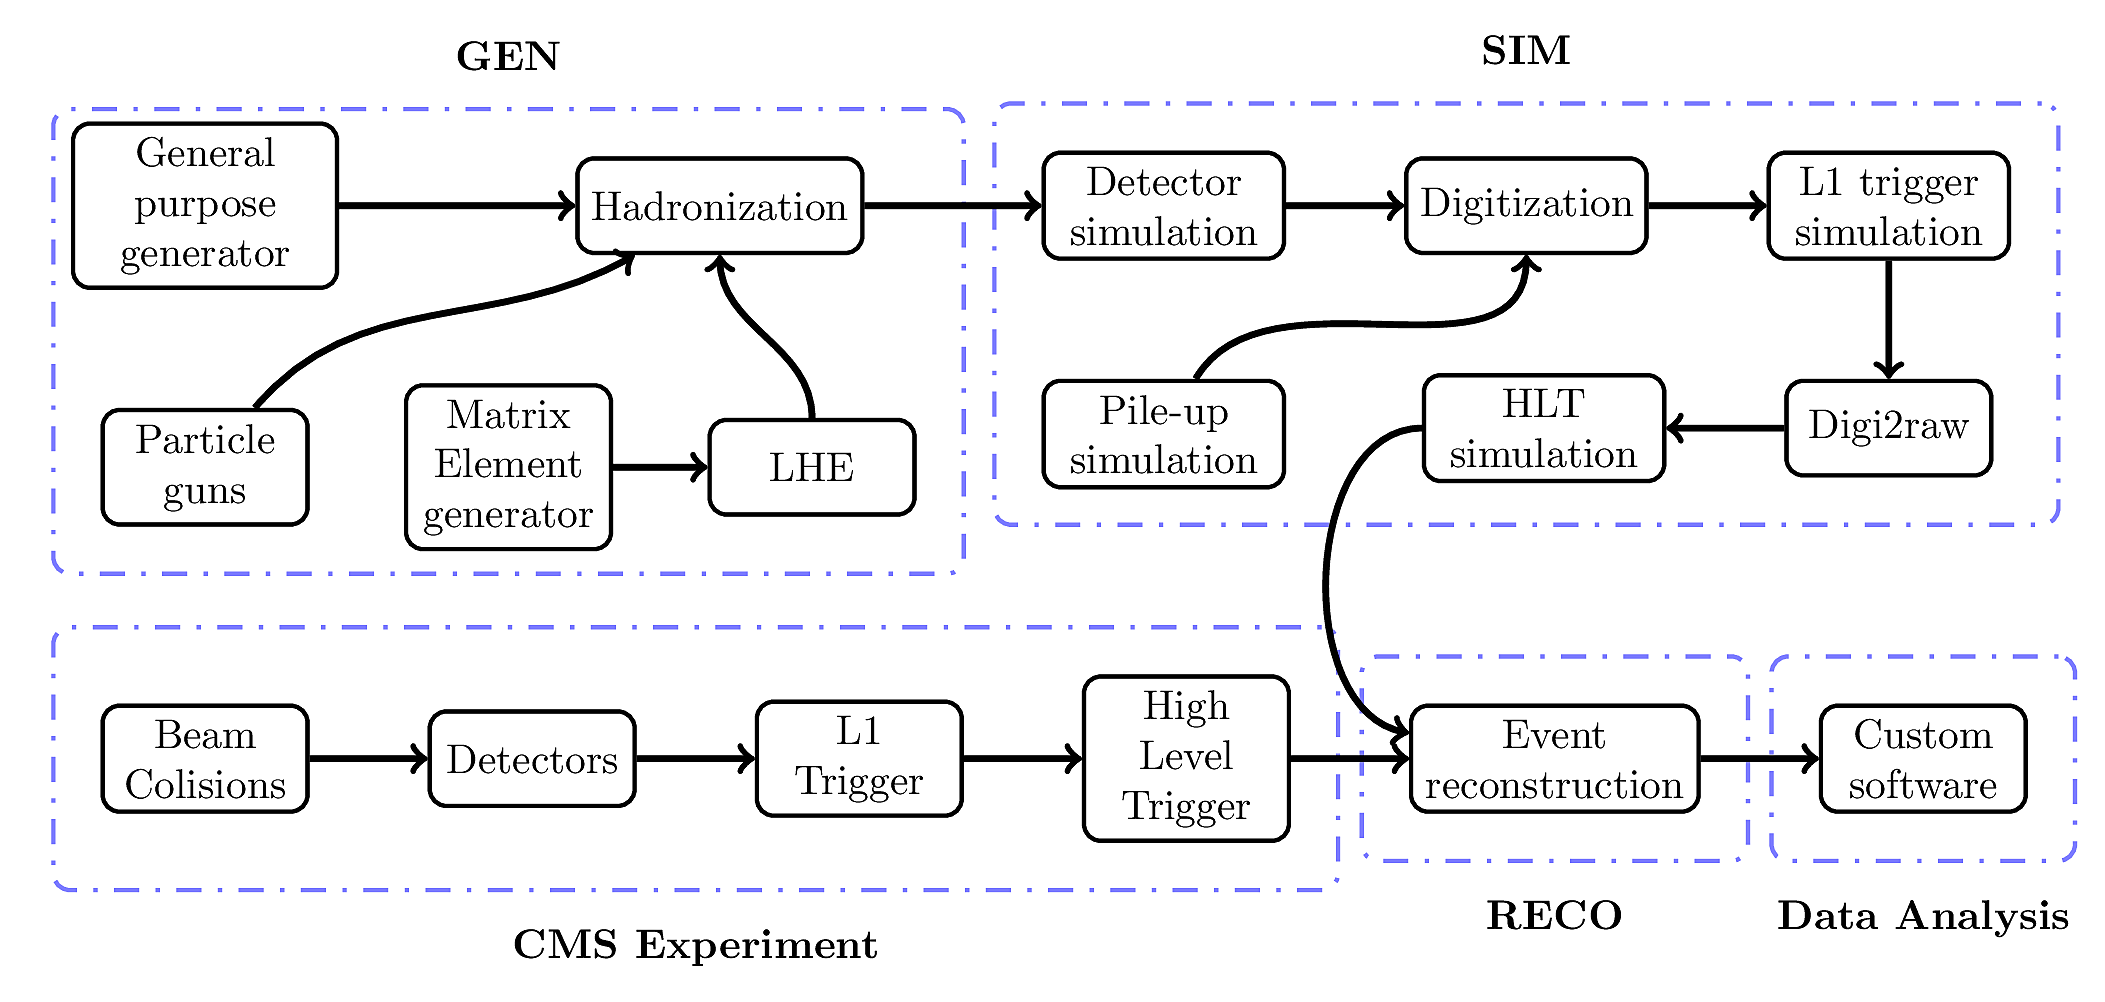
\includegraphics[width=0.9\textwidth]{fig/cms/mcgen_diagram.png}
    \caption[Diagram of the CMS collision data and simulation processing workflow]{
        Diagram of the CMS collision data and simulation processing workflow, from~\cite{CMSOpenDataMC}, for generating MC simulation showing the post-processing steps that are shared between MC simulation and real collision data. 
    }
    \label{fig:mcgen_diagram}
\end{figure}

\section{Event selection}
In order to isolate the signal, we must place a set of selections on our data that prefer events that look like signal. 
We do this in a particular order, however, because of the sheer size of our data: over the course of Run 2, the CMS Experiment collected over 200 PB of data! 
This data is processed and re-processed into more and more condensed descriptions of the same recorded events---the simulation is identically re-processed---but even at the smallest so-called ``data tier'', there is 200 TB of data and 900 TB of simulation (Fig.~\ref{fig:pp_to_nano}). 
Starting with triggers, progressively strict selections are placed that are optimized to prefer events that contain our signal. 
This process, orchestrated across 170 computing clusters in over 40 countries (i.e. 1000s of distributed CPUs), reduces 1.1 PB of data down to a few histograms. % TODO: cite WLCG website where these numbers are given

\begin{figure}[htb]
    \centering
    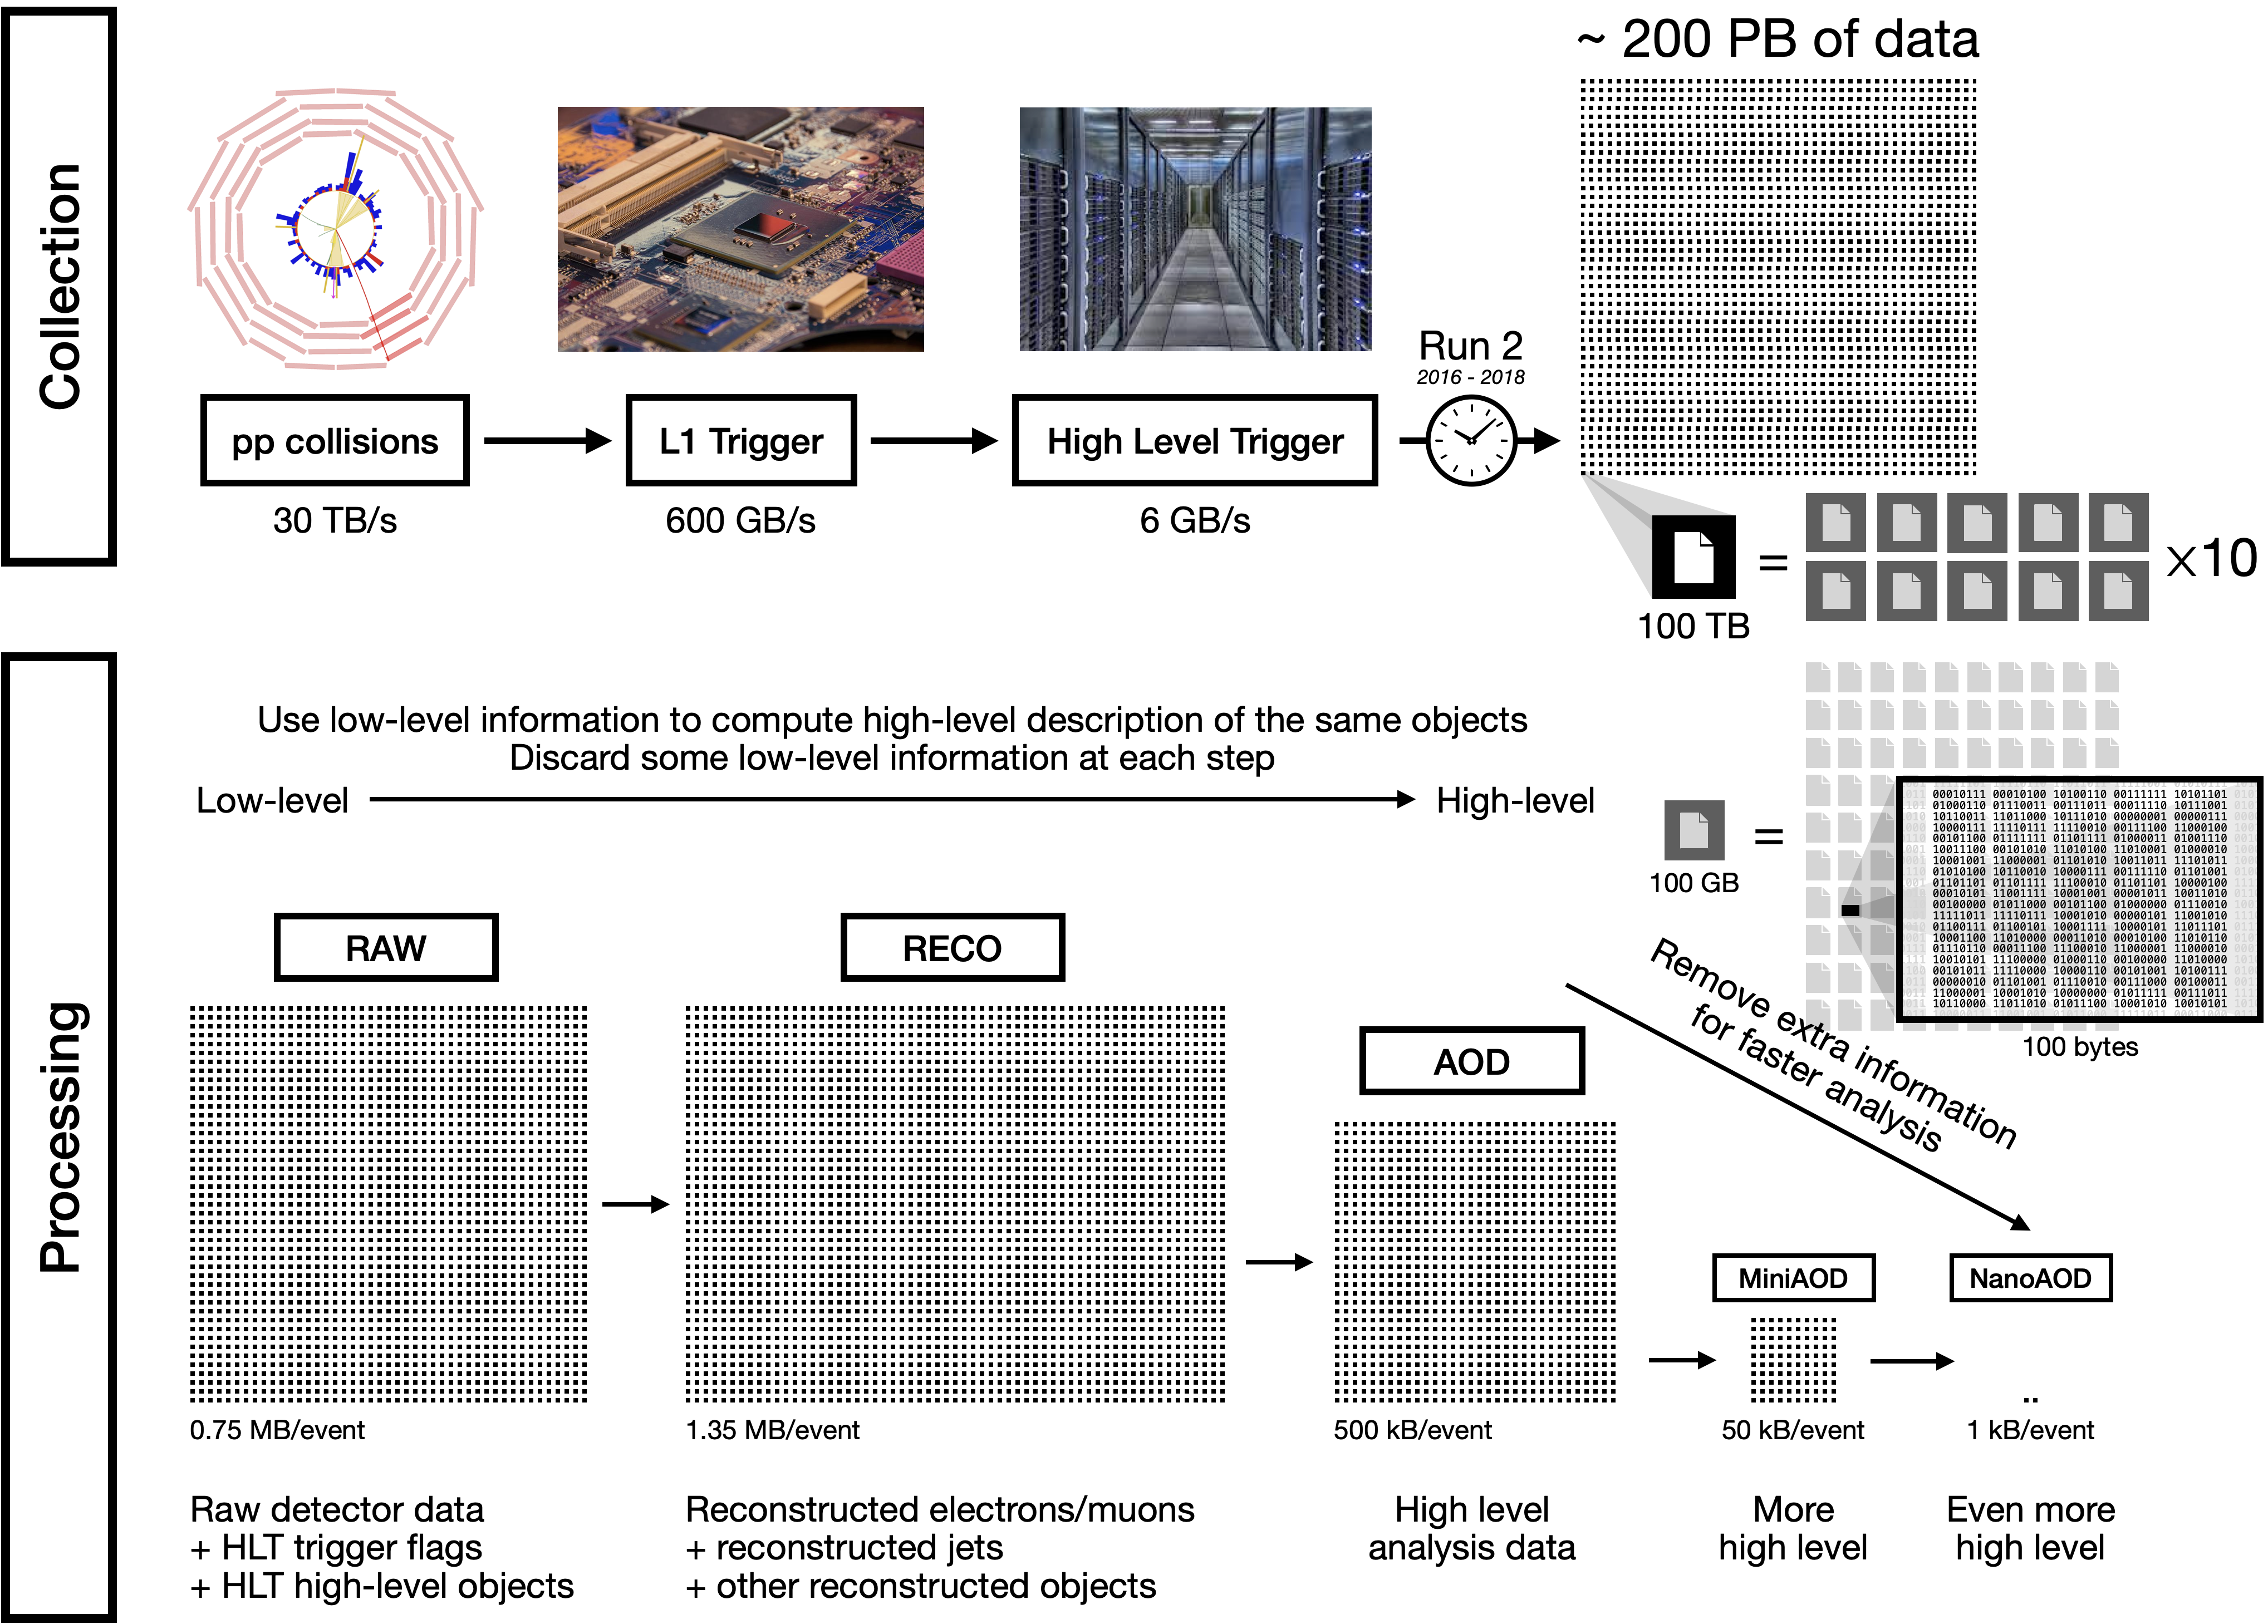
\includegraphics[width=0.95\textwidth]{fig/cms/pp_to_nano.png}
    \caption[Diagram of the evolution of CMS data from collection to post-processing into the data used in analysis]{
        Diagram of the evolution of CMS data from collection (top) to post-processing into the data used in analysis (bottom). 
        The 30 TB/s of data that are produced by the 40 MHz proton-proton collisions is reduced to 6 GB/s by the trigger system, which discards uninteresting events. 
        Over the course of Run 2, this yielded over 200 PB of recorded data that was then processed into different data ``tiers'' for further analysis. 
    }
    \label{fig:pp_to_nano}
\end{figure}

We first select the HLT paths most relevant to the chosen final state. 
For example, if the final state includes one lepton---say, from the leptonic decay of a \PW boson---then then we would select the single-lepton HLT paths. 
This isolates a portion of the petabytes of CMS data that are relevant for analysis. 
The HLT paths are also implemented in the simulation, so we will require that simulated events pass the same HLT paths as the data. 

Next, a series of selections are placed on the events passing the HLTs in order to narrow in on a set of events most relevant for analysis. 
For VBS Higgs boson analyses, these will select for at least two jets that look like VBS jets, and \Htobb reconstructed as one merged jet or two separate jets. 
These selections are referred to as the ``Preselection'' in this dissertation. 

The final set of selections are optimized using events that pass the Preselection. 
In the simplest analyses, like that presented in Chapter~\ref{ch:vbswh}, these selections will be on properties of each particle in the signal final state. 
Other analyses, like that presented in Chapter~\ref{ch:vbsvvh}, use these variables as input to a machine learning algorithm trained to select signal events. 
Ultimately, we select a final set of events that comprise the so-called ``signal region'' (Fig.~\ref{fig:nano_to_SR}). 
We will compare the number of actual collision events that enter this region to the number of events predicted by simulation. 
However, we must first derive the best possible estimate of the background in this region and compute all relevant systematic uncertainties. 

\begin{figure}[htb]
    \centering
    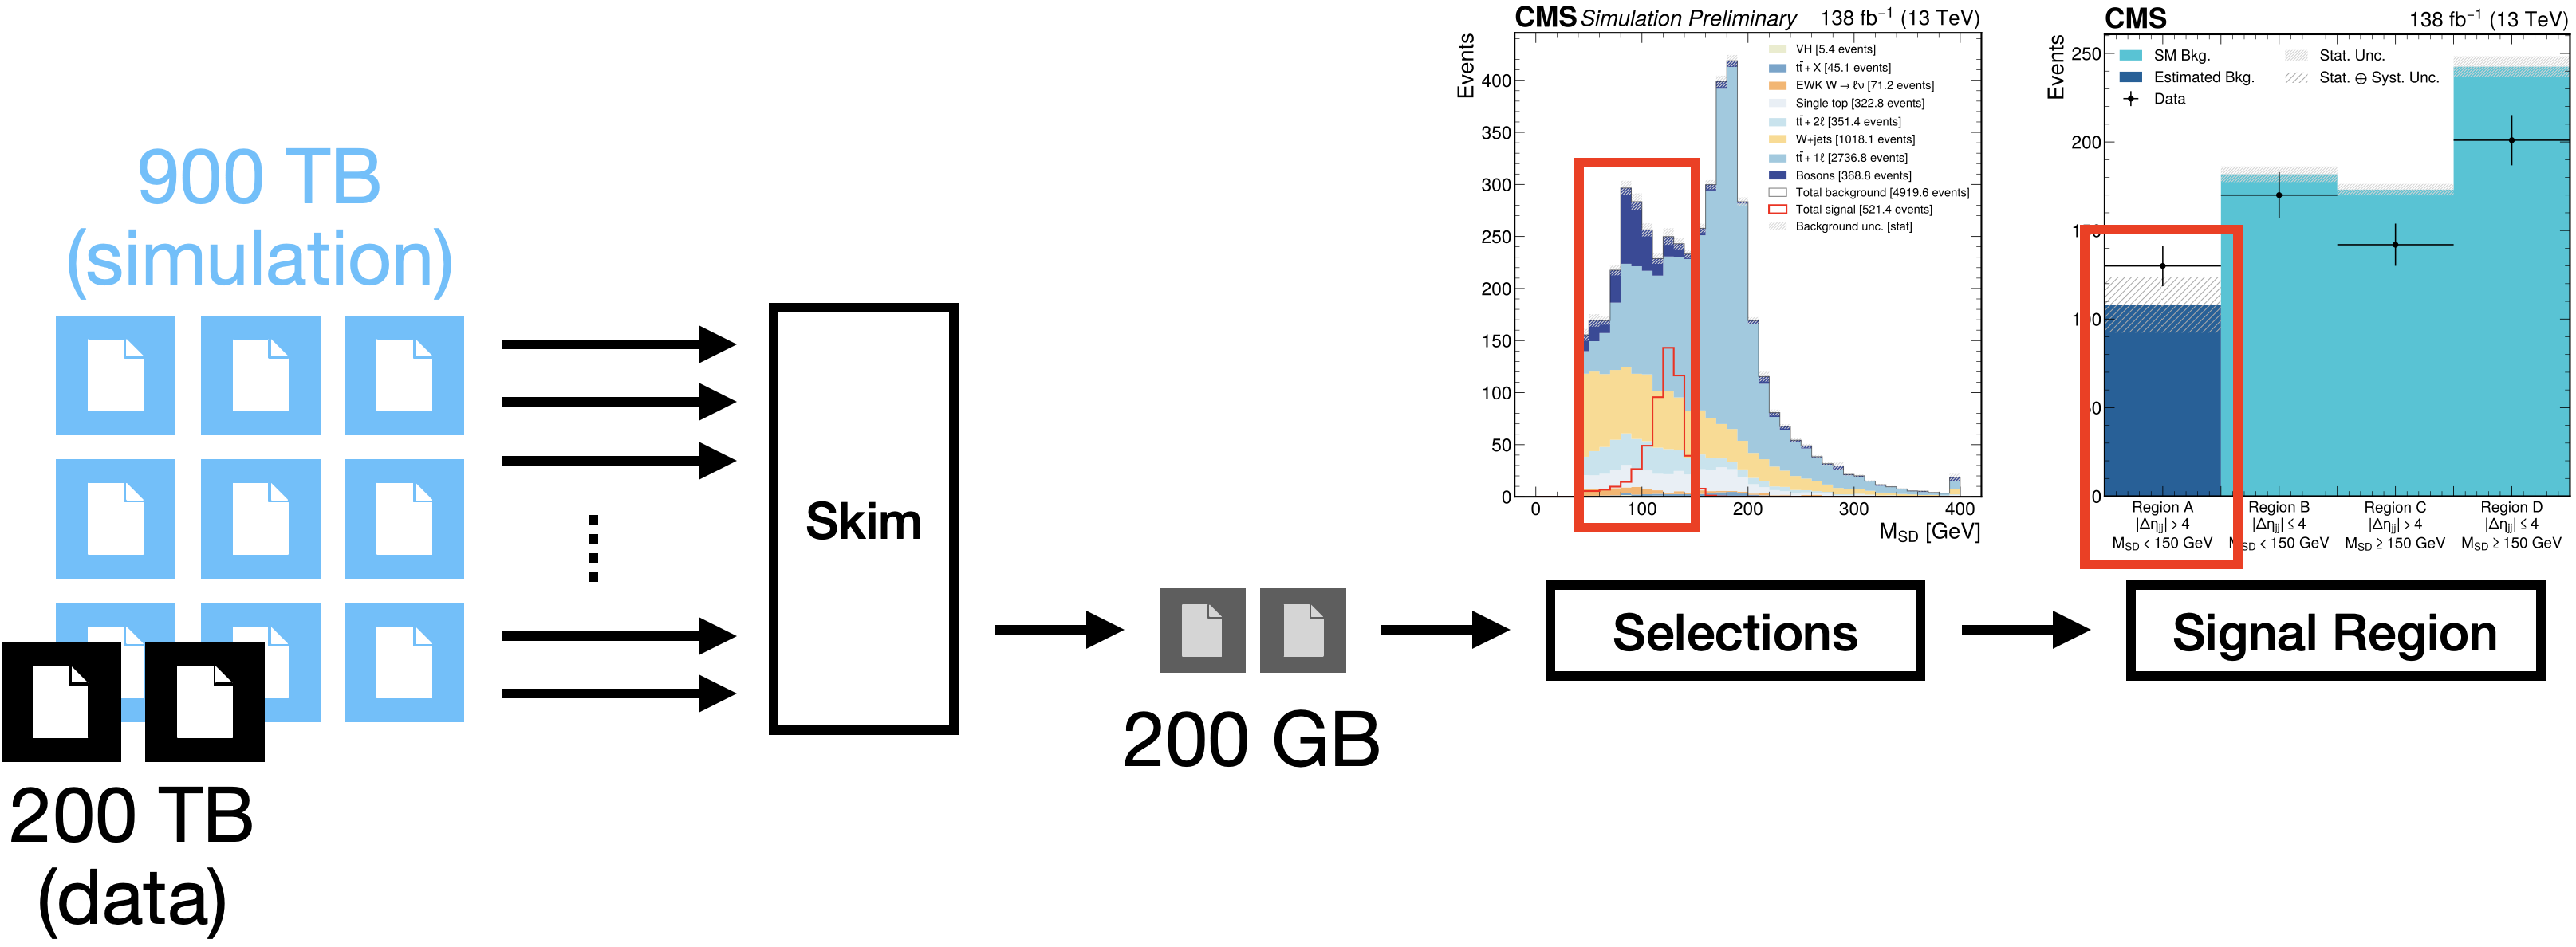
\includegraphics[width=0.95\textwidth]{fig/cms/nano_to_SR.png}
    \caption[Diagram of the data processing workflow for a typical measurement with CMS data]{
        Diagram of the data processing workflow for a typical measurement with CMS data. 
        Starting from NanoAOD (200 PB of real collision data, 900 PB of simulation), ``skimming'' jobs are distributed across thousands of GPUs, each taking a few NanoAOD files (around 1 GB each) and removing all of the unnecessary information. 
        Then, progressively strict selections are placed until the signal region is reached, wherein the measurement will be made. 
    }
    \label{fig:nano_to_SR}
\end{figure}

\section{Background estimation}
Although the predicted number of background events in the signal region can be taken directly from the simulation, the simulation is not perfect. 
Instead, there is a strategy---the famous ``ABCD'' method---in which only real data is used. 
The ABCD method entirely relies on there being two variables used to define the signal region that are decorrelated. 
For example, an analysis may have variables $x$ and $y$, where most of the signal has $x > 4$ and $y > 200$, whereas the background is concentrated near small values of $y$ and is uniformly distributed in $x$ (Fig.~\ref{fig:abcd}). 
In this case, if $x$ and $y$ are decorrelated, then for any value of $x$, the distribution of the background in $y$ will be the same and vice versa. 
Provided that this is true, we can look at real collision events with $x \leq 4$ and calculate
\begin{equation}
    f = \frac{\text{N events with }y > 200\text{ and }x \leq 4}{\text{N events with }y \leq 200\text{ and }x \leq 4}
\end{equation}
The distribution of $y$, and thereby the fraction $f$, should be identical to that for events with $x > 4$, since $x$ and $y$ are decorrelated, i.e. 
\begin{align}
    f' &= \frac{\text{N events with }y > 200\text{ and }x > 4}{\text{N events with }y \leq 200\text{ and }x > 4} \\
    f' &\approx f
\end{align}
Therefore, we can take the number of events with $x > 4$ and $y \leq 200$ and multiply it by $f$ to get the number of events we expect to have $x > 4$ and $y > 200$, i.e. 
\begin{equation}
    \bigg(\parbox{90pt}{\setsinglespacing\centering N events with\\$y > 200$ and $x > 4$}\bigg) 
    \approx 
    \bigg(\parbox{90pt}{\setsinglespacing\centering N events with\\$y \leq 200$ and $x > 4$}\bigg)
    \times 
    \frac{\text{N events with }y > 200\text{ and }x \leq 4}{\text{N events with }y \leq 200\text{ and }x \leq 4}
\end{equation}
For brevity, let $A$, $B$, $C$, and $D$, be the number of events with $y > 200$ and $x > 4$, $y \leq 200$ and $x > 4$, $y > 200$ and $x \leq 4$, and  $y \leq 200$ and $x \leq 4$, respectively. 
Then, the equation above becomes
\begin{equation}
    A \approx B\times\frac{C}{D}
\end{equation}
By estimating the background yield in the signal region in this way, we rely entirely on nature, which has no associated systematic uncertainties.

\begin{figure}[htb]
    \centering
    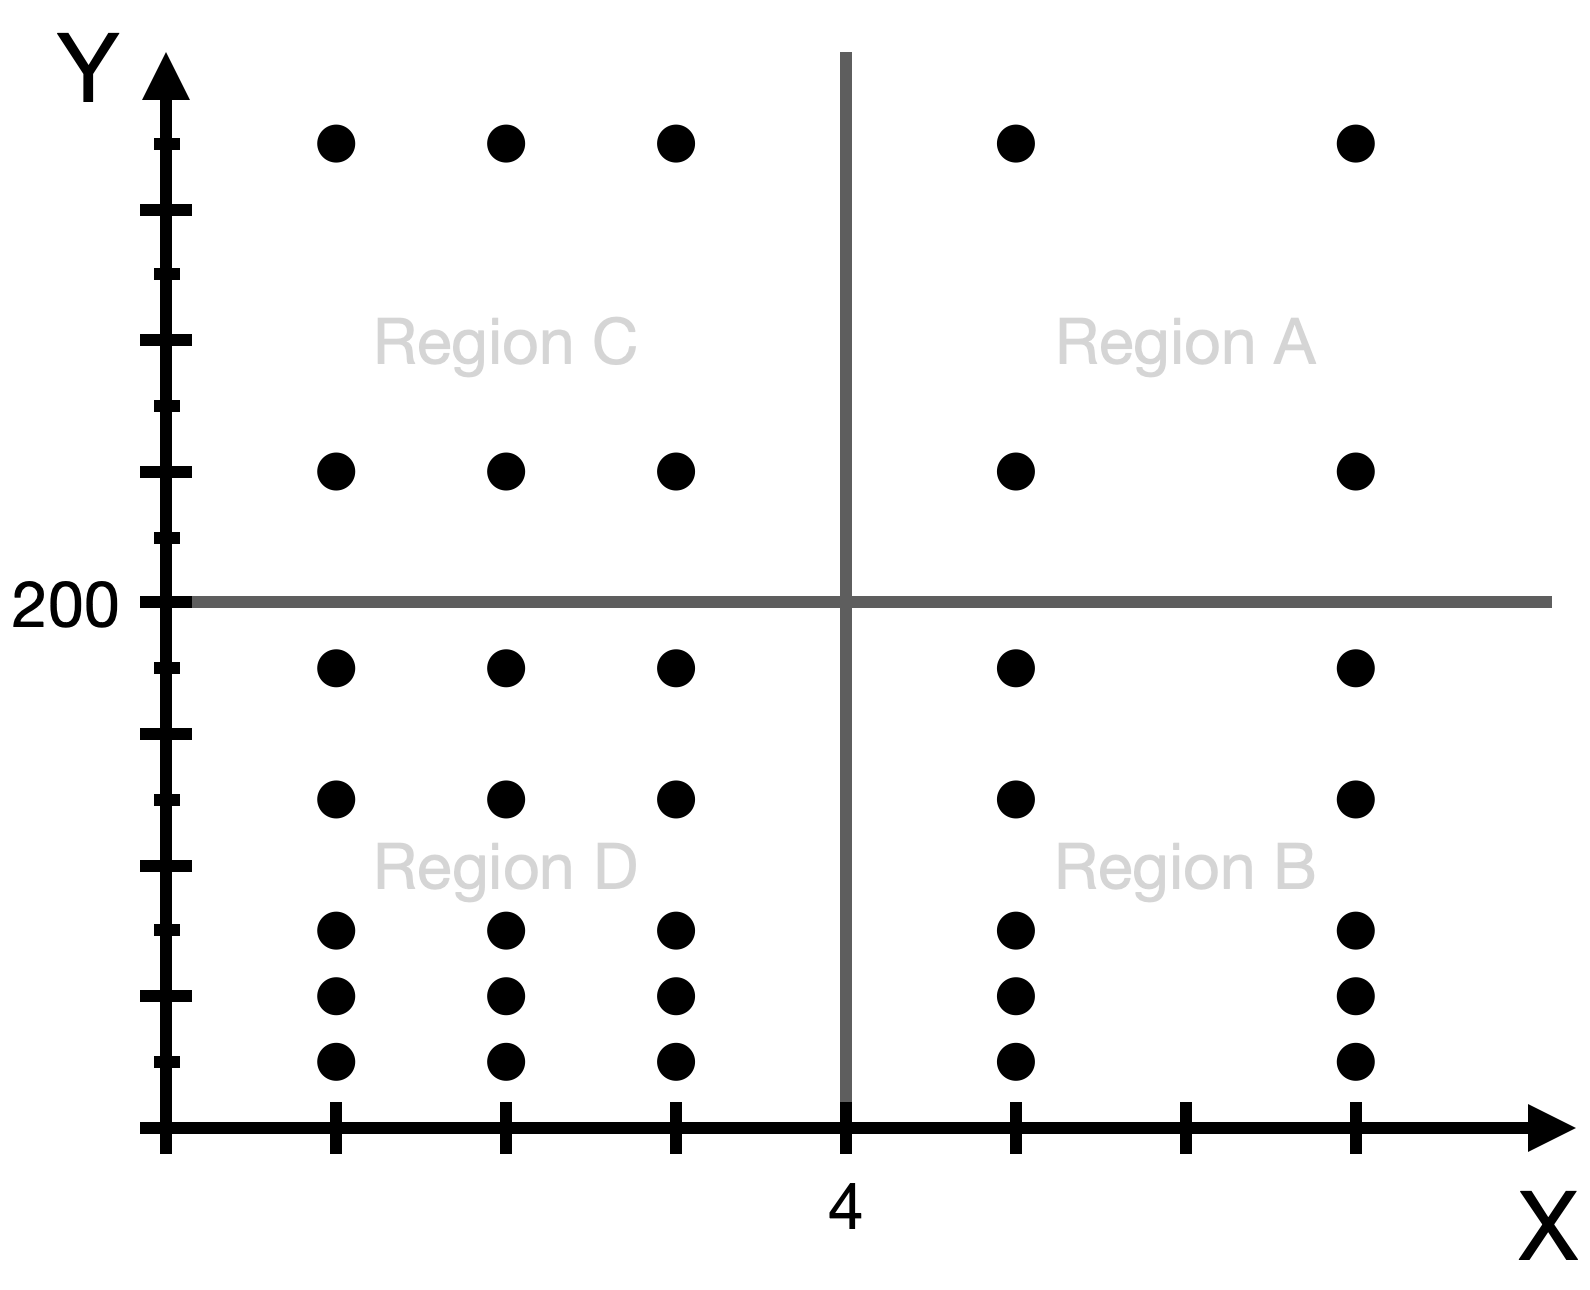
\includegraphics[width=0.45\textwidth]{fig/generic_abcd_cartoon.png}
    \caption[A generic ABCD configuration]{
        A generic ABCD configuration where selections on the quantities $x$ and $y$ are used to form the signal region (region A), and three ``control'' regions (regions B, C, and D) used to estimate the background in the signal region. 
        In the toy example shown, the method closes exactly for background (blue): $B\times C/D = 3 = A$. 
    }
    \label{fig:abcd}
\end{figure}

\section{Systematic uncertainties}
Since the background estimation strategy is data-driven, the systematic uncertainties on the simulation, which are numerous, only need to be evaluated for the signal yield. 
Systematic uncertainties in CMS statistical analysis come in two flavors: theoretical and experimental uncertainties. 
Sources of experimental uncertainty include the efficiency of the HLT, lepton identification, and \PQb tagging as well as the scale and resolution of the jet energies. 
For each of these sources, a correction has been derived to make simulation behave more like data. 
The HLT efficiency, for example, can be directly compared to data; 90\% pass in simulation, versus 95\% in data, then each passing event can be considered instead as 1.056 events, forcing the overall yields to match. 
Then, the associated experimental uncertainty is quantified by taking the correction, varying it up and down by one standard deviation\footnotemark{}, and assessing the impact on the final measurement. 
\footnotetext{This uncertainty is derived differently for each correction.}
Theoretical uncertainties, meanwhile, are quantified by varying parameters of the simulation up and down and assessing the impact on the final measurement. 

\section{Statistical interpretation} % quote PDG on section statistics or something
The analyses presented in this dissertation are counting experiments. 
That is, for the final result, we take the expected signal yield \Asignal and predicted background yield \AdataPred in the signal region and compare them to the yield of real collision events \Adata. 
Intuitively, if $\Adata = \AdataPred$, then our signal most likely does not exist in nature; conversely, if $\Adata = \Asignal+\AdataPred$, then we have just confirmed that our signal does exist. 
But what can we say if \Adata is somewhere between \AdataPred and $\Asignal+\AdataPred$? 
We have also just enumerated through the many systematic uncertainties on \Asignal and \AdataPred that affect our ability to make this comparison exactly. 
For example, \AdataPred may have, by chance, fluctuated upward by just enough to make it seem as though our signal exists---or worse, it may have fluctuated downward and made us think our signal is not real. 
Using statistics, we can make a more precise statement about our measurement, taking all of the uncertainties into account. 

\subsection{Probability and likelihood}
The \textit{probability} that we observe $n$ events in our signal region given the expected yield $\lambda$ follows Poisson statistics:
\begin{equation}
    P(n|\lambda) = \frac{\lambda^n e^{-\lambda}}{n!}
\end{equation}
In our analysis, $\lambda = \mu s + b$, or some fixed number $\mu$ times the signal yield $s$ plus the background yield $b$. 
The number $\mu$ is called the ``signal strength'' because $\mu s$ represents different scenarios: e.g. the signal does not exist ($\mu = 0$), the signal does exist ($\mu = 1$), the signal is 50\% smaller than our model expected ($\mu = 0.5$), and so on. 
Revising our equation, we obtain
\begin{equation}
    P(n|\mu, s, b) = \frac{(\mu s + b)^n e^{-(\mu s + b)}}{n!}
\end{equation}
We need a slightly different formulation, however, because we have already observed $n$ events. 
That is, we already know the \textit{outcome} of our experiment, and we are trying to explain that outcome based on the \textit{parameters} of the underlying statistical model---Poisson statistics in this case. 
In other words, we need the probability that the signal strength is some number $\mu$, given the yields $n$, $s$, and $b$. 
We call this the likelihood $L$, or
\begin{equation}
    L(\mu) = \frac{(\mu s + b)^n e^{-(\mu s + b)}}{n!}
\end{equation}
Importantly, $P$ and $L$ are related, and thus superficially similar, but they are distinct quantities (Fig.~\ref{fig:prob_vs_like}). 

\begin{figure}[htb]
    \centering
    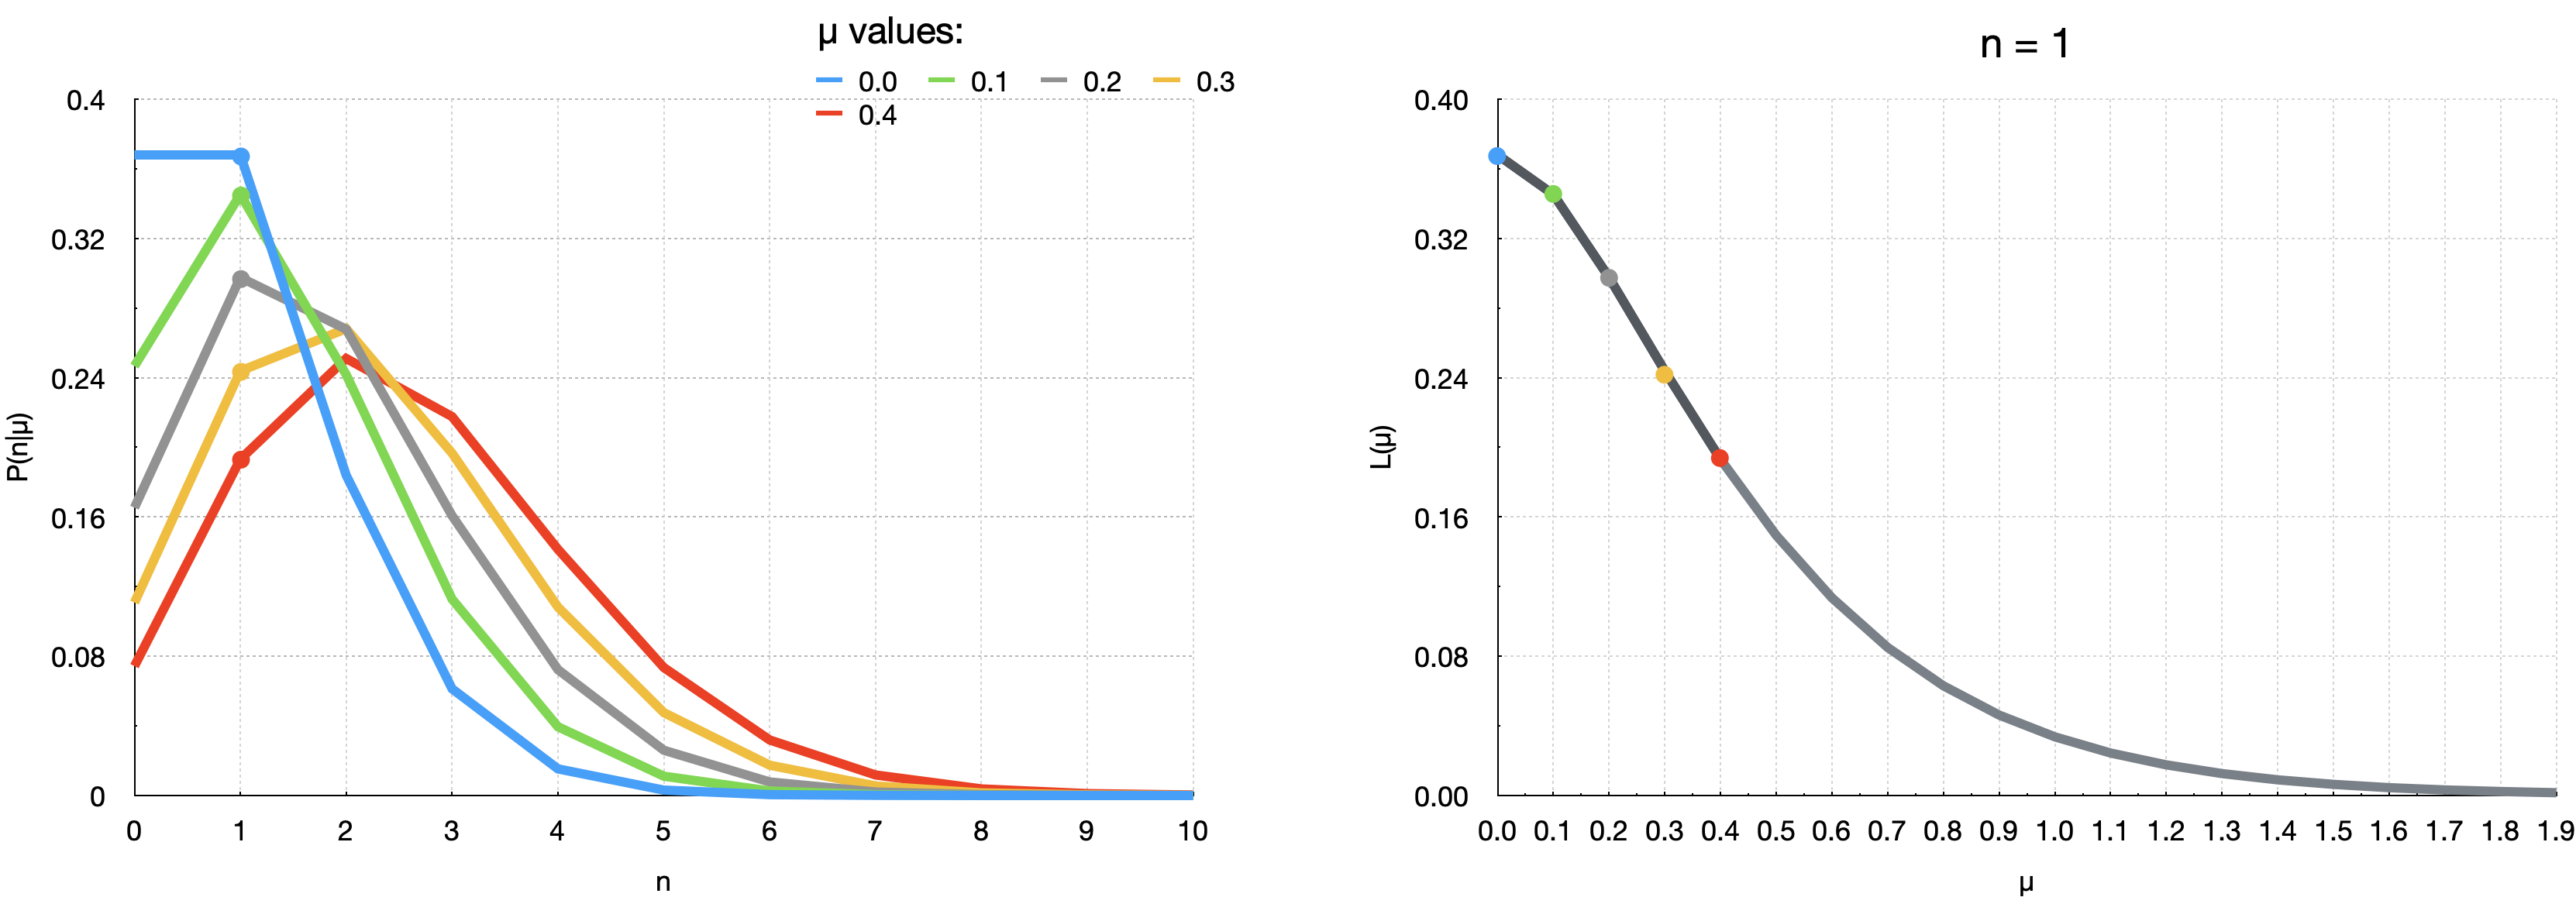
\includegraphics[width=0.95\textwidth]{fig/stats/prob_vs_like.png}
    \caption[The probability and likelihood]{
        The probability for different values of $\mu$ (left) and the likelihood for $n = 1$ (right), showing how $L(\mu)|_{n=1}$ is given by computing $P(1|\mu)$. 
    }
    \label{fig:prob_vs_like}
\end{figure}

\subsection{Maximum likelihood estimate}
Our task can now be expressed in the proper language of statistics: the most probable value of $\mu$ given $n$, $s$, and $b$ is given by the maximum of the likelihood $L(\mu)$. 
Fortunately, this is basic calculus: take the derivative of $L$ with respect to $\mu$, set it equal to zero, and solve. 
For simplicity, we will instead consider $q(\mu) = -2\ln{L(\mu)}$:
\begin{align}
    q(\mu) &= -2[n\ln(\mu s + b) - (\mu s + b) - \ln{(n!)}] \nonumber \\
    \frac{\partial q}{\partial \mu} &= 1 - \frac{n}{\mu s + b}\qquad\text{where }\frac{\partial q}{\partial \mu}\bigg|_{\mu=\hat{\mu}} \equiv 0 \nonumber \\
    0 &= 1 - \frac{n}{\hat{\mu} s + b} \nonumber \\
    \hat{\mu} &= \frac{n - b}{s}
\end{align}
In our simple setup, this is rather intuitive: plugging $\hat{\mu}$ into $\mu s + b$ gives $n$ exactly. 
We can now easily compute $\hat{\mu}$ for a given value of $n$, $s$, and $b$, but we must also declare how confident we are in our measurement.

Assuming the likelihood is approximately Gaussian\footnotemark{} with an amplitude $\mathcal{N}$ and standard deviation of $\sigma_\mu$---which is true for large $n$ (Fig.~\ref{fig:like_gauss_approx})---we can express $L(\mu)$ as
\footnotetext{For non-physicists, this is referring to a normal distribution or bell curve.}
\begin{equation}
    L(\mu) \approx \mathcal{N}e^{\frac{-(\mu - \hat{\mu})^2}{-2\sigma^2_\mu}}
\end{equation}
For convenience, we again consider a more useful quantity $q(\mu)$:
\begin{equation}
    q(\mu) = -2\ln\frac{L(\mu)}{L(\hat{\mu})} = \bigg(\frac{\mu - \hat{\mu}}{\sigma_\mu}\bigg)^2
\end{equation}
where $\sqrt{q(\mu)}$ can be interpreted as the number of standard deviations away $\mu$ is from $\hat{\mu}$. 
In other words, for a given value of $\hat{\mu}$, we can now express the range of possible values of $\mu$ within 1, 2, or more standard deviations (Fig.~\ref{fig:CL_examples})---this is called a confidence interval. 
If, for example, we had 413 expected signal events, 128 predicted background events, and observed 550 real events, then we could say that the signal strength was measured to be within the 95\% confidence interval $[0.88, 1.10]$. 

\begin{figure}[htb]
    \centering
    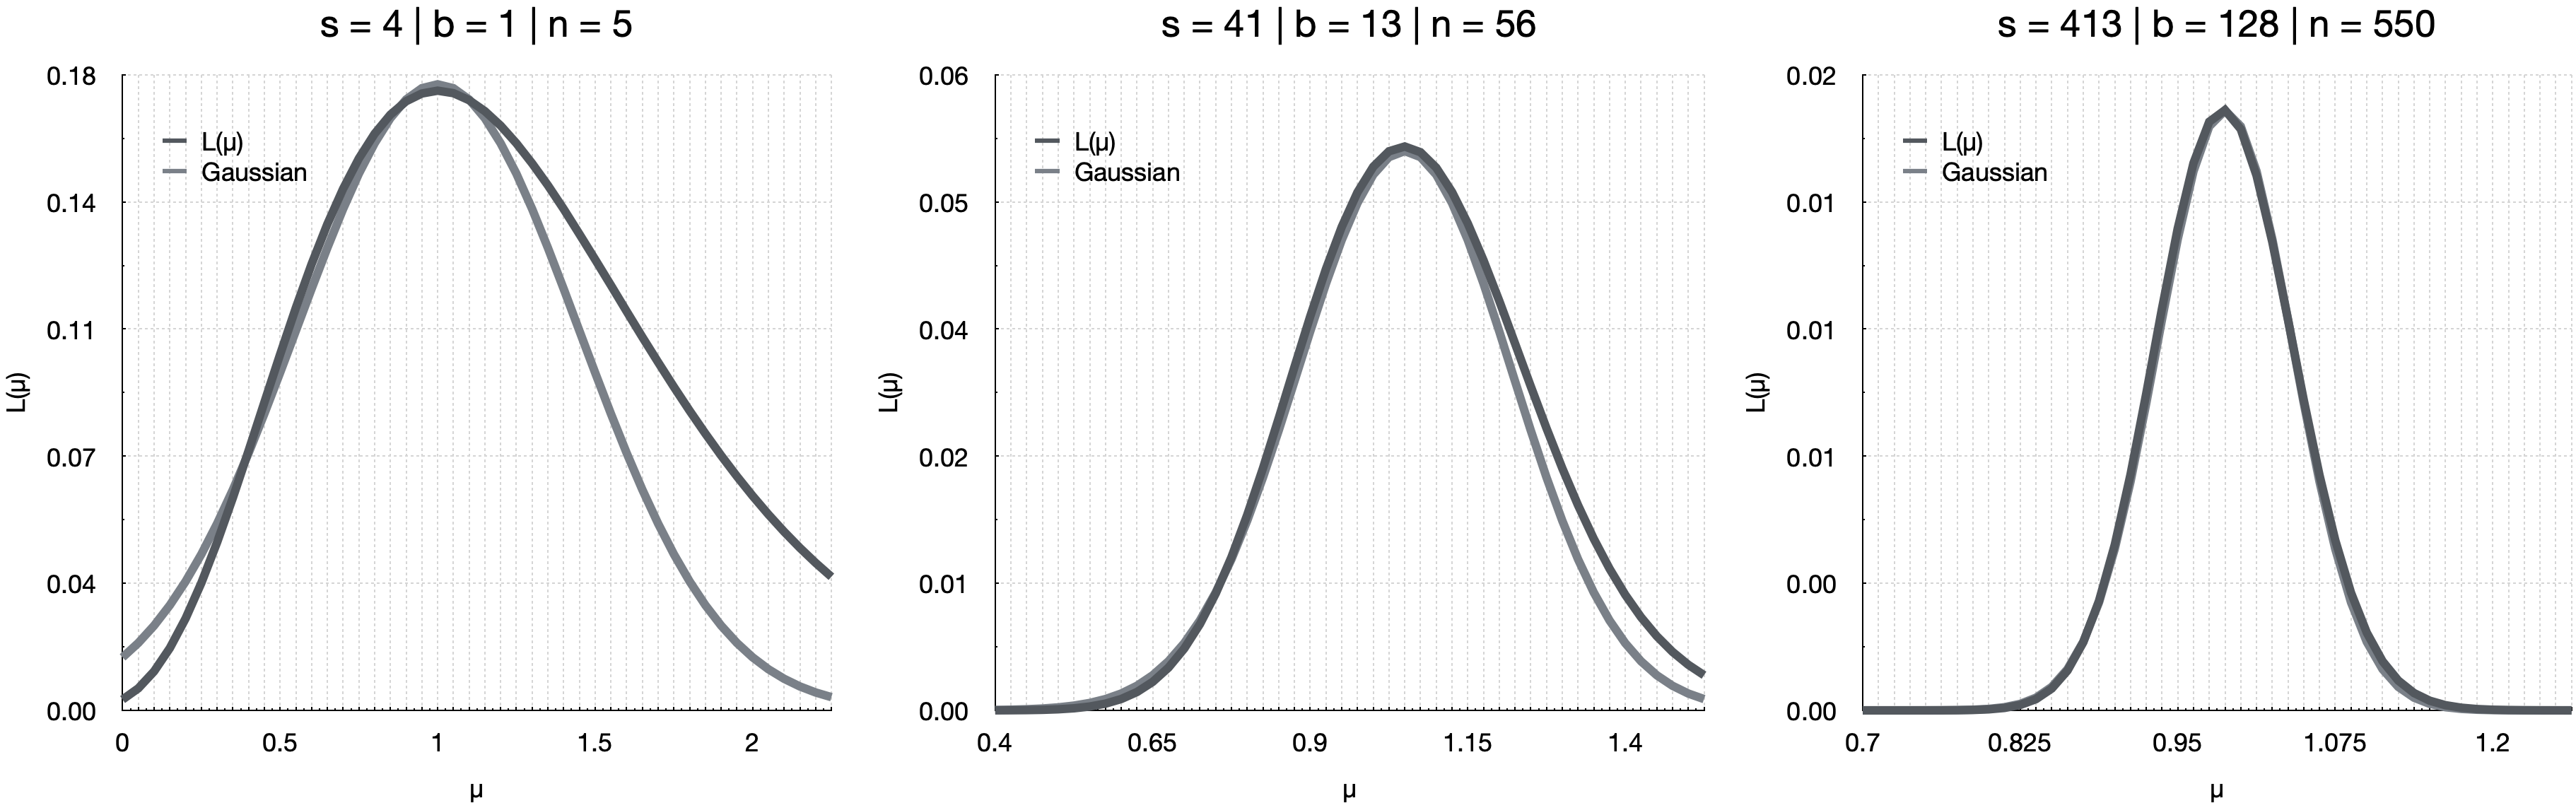
\includegraphics[width=0.95\textwidth]{fig/stats/like_gauss_approx.png}
    \caption[The likelihood with the Gaussian approximation of the likelihood overlaid]{
        The likelihood with the Gaussian approximation of the likelihood overloaded for different values of $n$, showing poor agreement for small $n$ (left), decent agreement for $n = 56$, and good agreement for $n = 550$.
    }
    \label{fig:like_gauss_approx}
\end{figure}

\begin{figure}[htb]
    \centering
    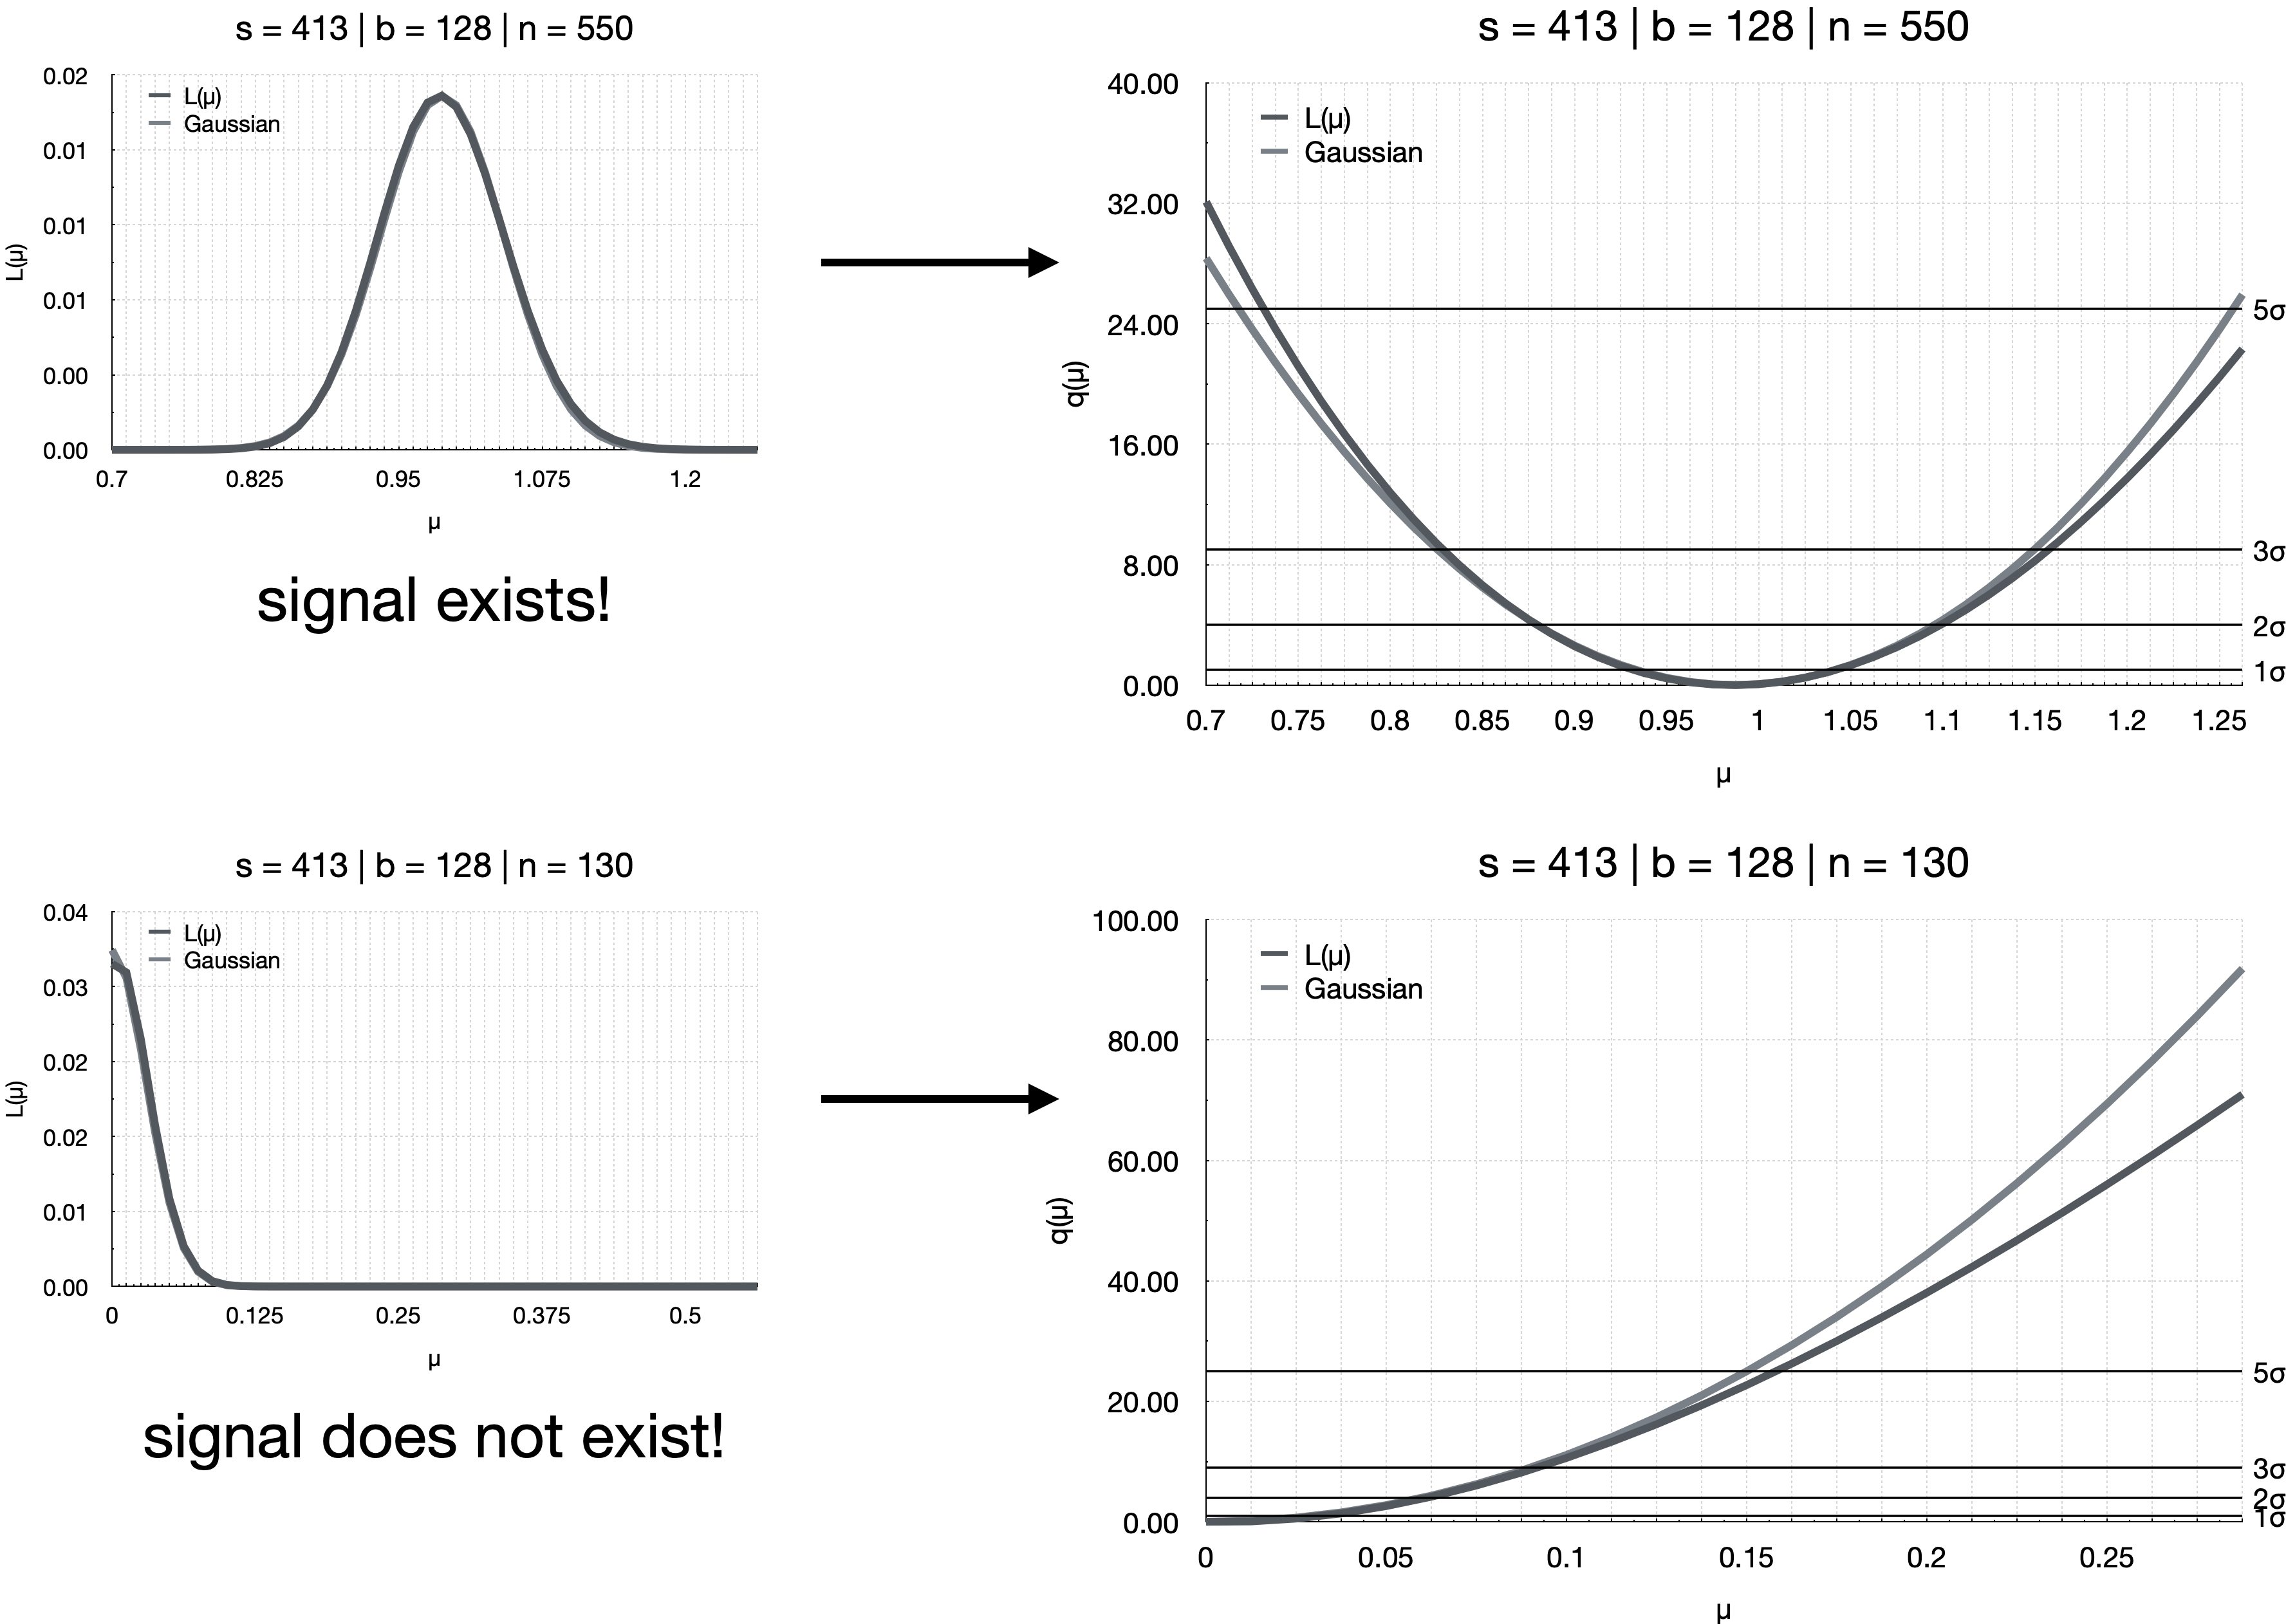
\includegraphics[width=0.95\textwidth]{fig/stats/CL_examples.png}
    \caption[The likelihood and confidence interval plotted for the ``signal exists'' and ``signal does not exist'' scenarios]{
        The likelihood (left) and confidence interval (right) plotted for two different scenarios: $n \approx s$, or the signal exists, (top) and $n \approx b$, or the signal does not exist (bottom). 
        In the first scenario, the signal strength is measured to be within $[0.88, 1.10]$ at the 95\% CL, whereas in the other scenario, it is measured to be within $[0, 0.06]$ at the 95\% CL.
    }
    \label{fig:CL_examples}
\end{figure}

So far, we have not considered the uncertainty in $s$ or $b$, which are critical to the accuracy of our confidence interval. 
Focusing on the signal yield, we can decompose $s$ into multiple components:
\begin{equation}
    s = \big(\underbrace{\substack{\text{detector} \\ \text{acceptance}}}_A\big)
        \times\big(\underbrace{\substack{\text{detection} \\ \text{efficiency}}}_\epsilon\big)
        \times\big(\underbrace{\substack{\text{integrated} \\ \text{luminosity}}}_\mathcal{L}\big)
        \times\big(\underbrace{\substack{\text{cross} \\ \text{section}}}_\sigma\big)
\end{equation}
At CMS, we are able to measure the integrated luminosity for all of Run 2 with an uncertainty of around 1.6\%. 
If we wanted to include this uncertainty in our statistical analysis, we could rewrite the luminosity term \Lumi
\begin{equation}
    s = A\epsilon\Lumi_0(1 + 1.016)^\eta\sigma
\end{equation}
where $\Lumi_0$ is the measured value of the integrated luminosity and $\eta$ is typically a Gaussian-distributed number between 0 and 1. 
Before we compute our confidence interval, we must find some $\hat{\eta}(\mu)$ that minimizes $q(\mu, \nu(\mu))$. 
For each systematic uncertainty in our analysis, we add another ``nuisance parameter'' that must first be minimized before the final result is produced. 
In this dissertation, this operation---along with the maximum likelihood estimation---is performed by the \COMBINE tool~\cite{CombinePaper}. 
